\documentclass[aspectratio=169]{beamer}
\usepackage{hyperref}
\usepackage[T1]{fontenc}
\usepackage[spanish]{babel}
\usepackage{csquotes}
\usepackage{tribhuvan}

\AtBeginSection[]{
  \begin{frame}[plain]
    \vfill
    \begin{center}
      {\LARGE\bfseries \insertsectionhead}
    \end{center}
    \vfill
  \end{frame}
}
\AtBeginSubsection[]{}

\author{Rodrigo Pérez Rodríguez}
\title{Tecnologías Robóticas para la Discapacidad Intelectual}
\subtitle{Introducción a la robótica social y asistencial}
\date{}
\setbeamertemplate{date}{}

\newcommand{\originalpagefigure}[1]{}

\begin{document}

\begin{frame}
  \titlepage
\end{frame}

\begin{frame}{Contenido}
  \tableofcontents
\end{frame}

% Página original 2
\section{Historia}

% Página original 3
\begin{frame}{Popularidad de los robots}
  \small
  \begin{columns}[T,onlytextwidth]
    \begin{column}{0.62\textwidth}

        \begin{itemize}
          \item Mitificación propiciada por la literatura y el cine de ciencia ficción
          \item Pero la realidad es bien diferente
        \end{itemize}
    \end{column}
    \begin{column}{0.38\textwidth}
      \centering
      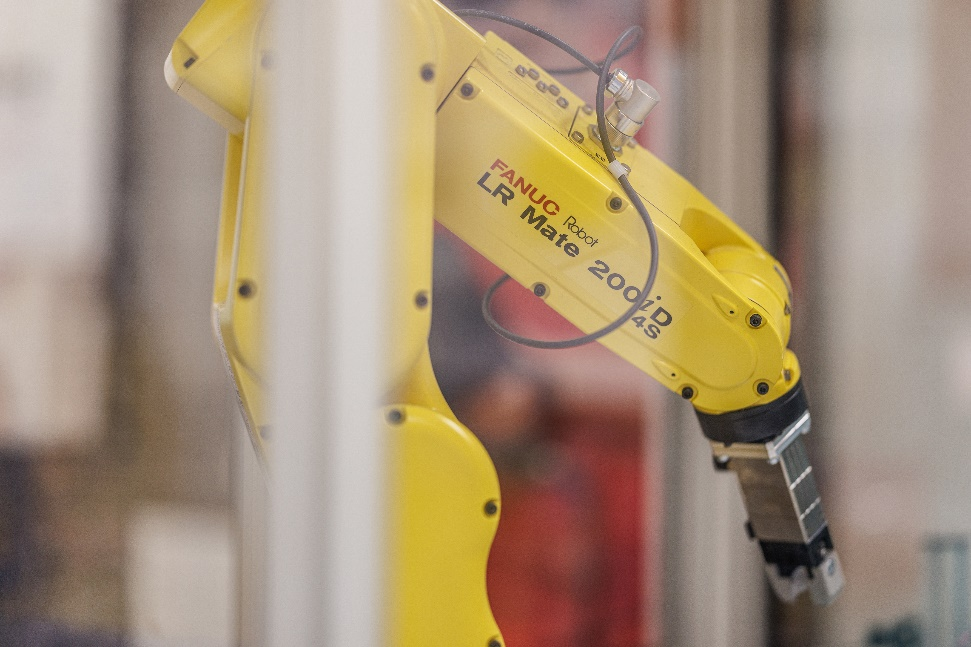
\includegraphics[width=0.97\linewidth,height=0.30\textheight,keepaspectratio]{images/intro/by_slide/s03_popularidad-de-los-robots_img01.jpeg}
      \par\vspace{0.02\textheight}
      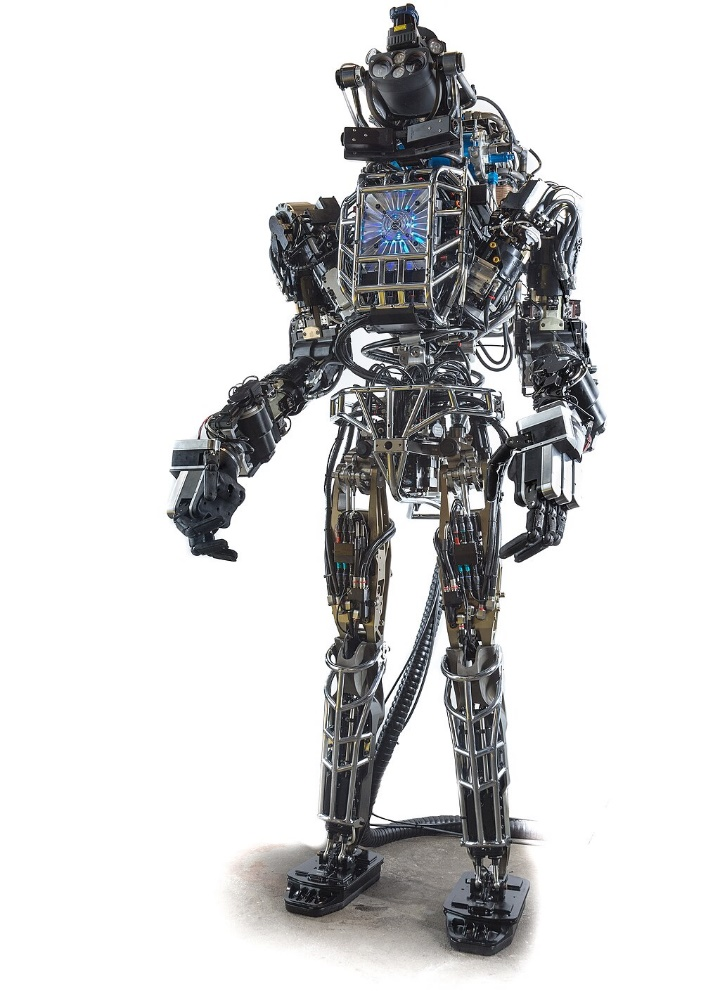
\includegraphics[width=0.97\linewidth,height=0.30\textheight,keepaspectratio]{images/intro/by_slide/s03_popularidad-de-los-robots_img02.jpeg}
    \end{column}
  \end{columns}
\end{frame}

% Página original 4
\begin{frame}{Popularidad de los robots}
  \small
  \begin{itemize}
    \item Isaac Asimov (1920-1992) es quizá el máximo impulsor de la palabra ‘robot’, y quizá también de la palabra ‘robótica’
    \item Enunció, en su obra ‘Bóvedas de acero’ (1953), las 3 leyes de la robótica:
    \begin{itemize}
      \item Un robot no puede perjudicar a un ser humano, ni con su inacción permitir que un ser humano sufra daño
      \item Un robot ha de obedecer las órdenes recibidas de un ser humano, excepto si tales órdenes entran en conflicto con la primera ley
      \item Un robot debe proteger su propia existencia mientras tal protección no entre en conflicto con la primera o segunda ley
    \end{itemize}
  \end{itemize}
\end{frame}

% Página original 5
\begin{frame}{Autómatas}
  \small
  \begin{columns}[T,onlytextwidth]
    \begin{column}{0.62\textwidth}
      \begin{itemize}
        \item El ser humano, a lo largo de la historia, se ha sentido fascinado por aquellos dispositivos capaces de imitar a los seres vivos $\rightarrow$ autómatas
      \end{itemize}
    \end{column}
    \begin{column}{0.38\textwidth}
      \centering
      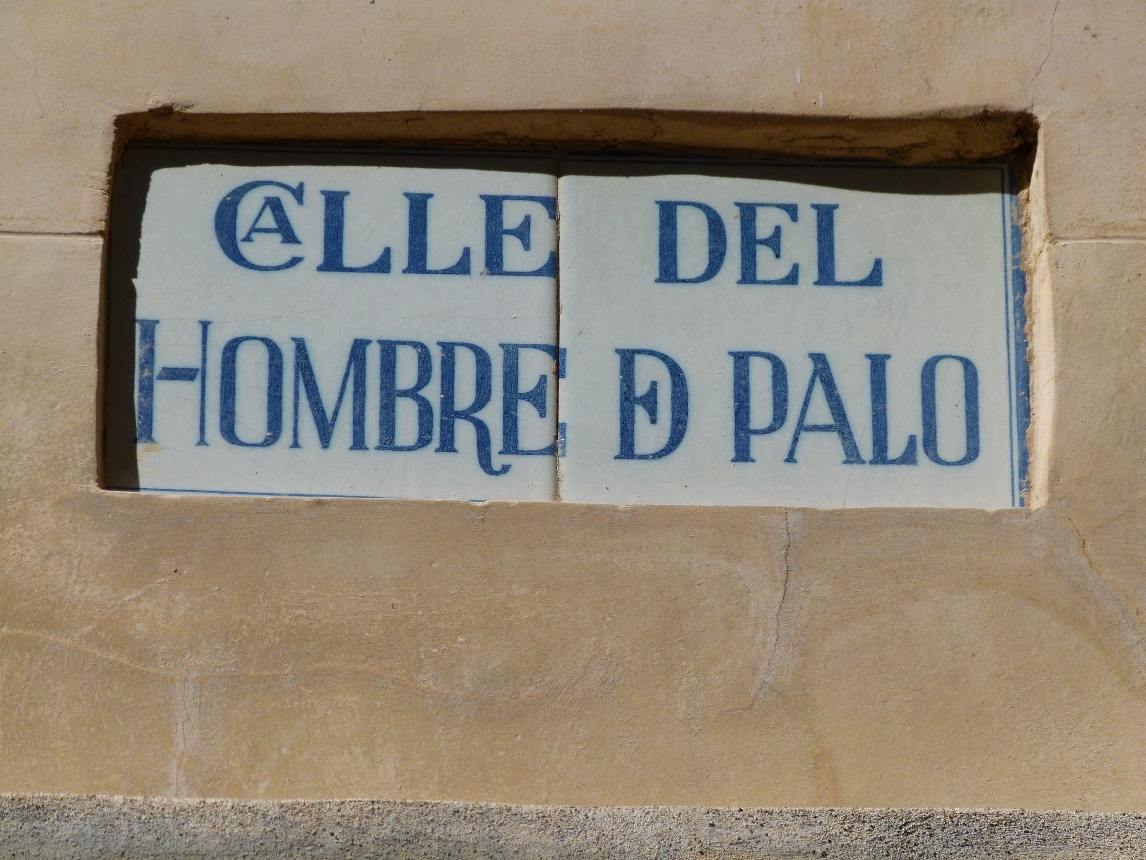
\includegraphics[width=0.97\linewidth,height=0.62\textheight,keepaspectratio]{images/intro/by_slide/s05_automatas_img01.jpeg}
    \end{column}
  \end{columns}
\end{frame}

% Página original 6
\begin{frame}{Algunos autómatas históricos}
  \small
  \begin{columns}[T,onlytextwidth]
    \begin{column}{0.62\textwidth}
      \begin{itemize}
        \item Gallo de la catedral de Estrasburgo
        \begin{itemize}
          \item 1352, autor desconocido
          \item Operativo hasta 1789
          \item Aparecía con otras figuras representando los apóstoles
          \item Movía las alas, levantaba la cabeza y cacareaba 3 veces
        \end{itemize}
      \end{itemize}
    \end{column}
    \begin{column}{0.38\textwidth}
      \centering
      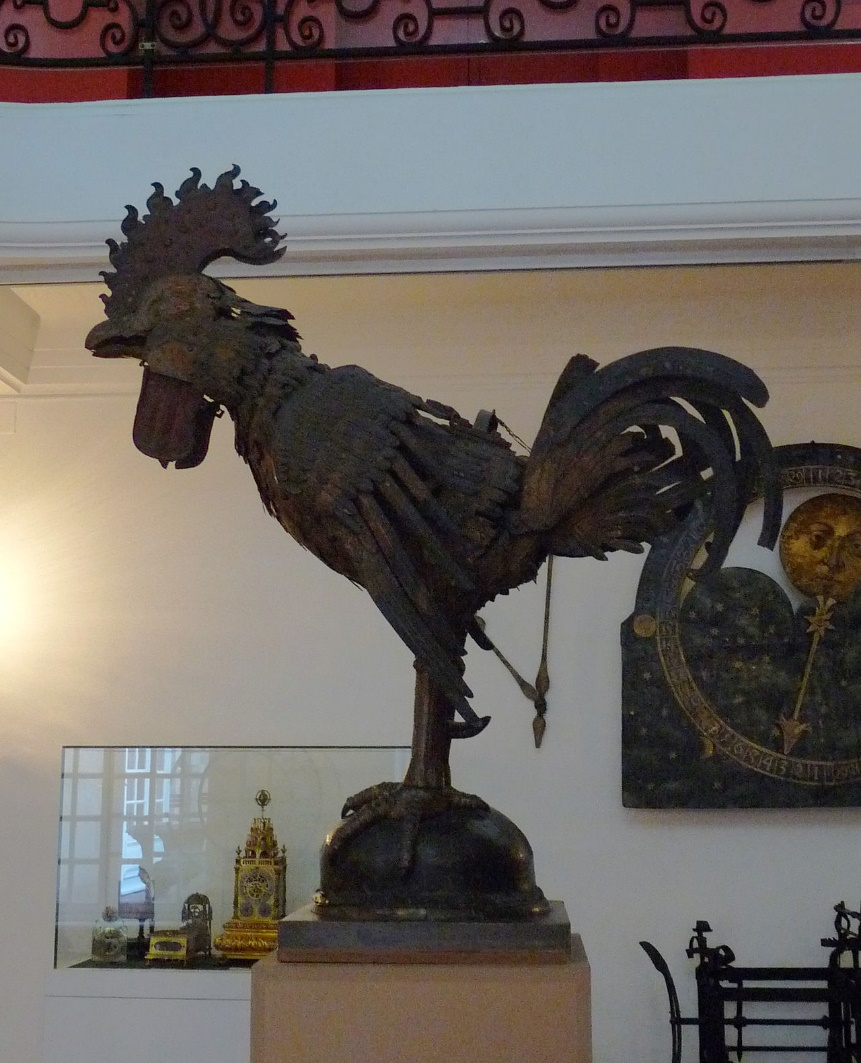
\includegraphics[width=0.97\linewidth,height=0.62\textheight,keepaspectratio]{images/intro/by_slide/s06_algunos-automatas-historicos_img01.jpeg}
    \end{column}
  \end{columns}
\end{frame}

% Página original 7
\begin{frame}{Algunos autómatas históricos}
  \small
  \begin{columns}[T,onlytextwidth]
    \begin{column}{0.62\textwidth}

        \begin{itemize}

          \item Hombre de palo
          \begin{itemize}
            \item 1525, Juanelo Turriano
            \item Humanoide
            \item Programado para andar unos pasos moviendo los ojos y la boca
            \item Con una mano sujetaba un crucifijo y con la otra se golpeaba el pecho
          \end{itemize}
          
          \item Pato
          \begin{itemize}
            \item 1738, Jaques de Vaucanson
            \item Pato de cobre que comía, bebía, graznaba, movía las alas
            \item Digería la comida como un pato real
          \end{itemize}
        \end{itemize}
    \end{column}
    \begin{column}{0.38\textwidth}
      \centering
      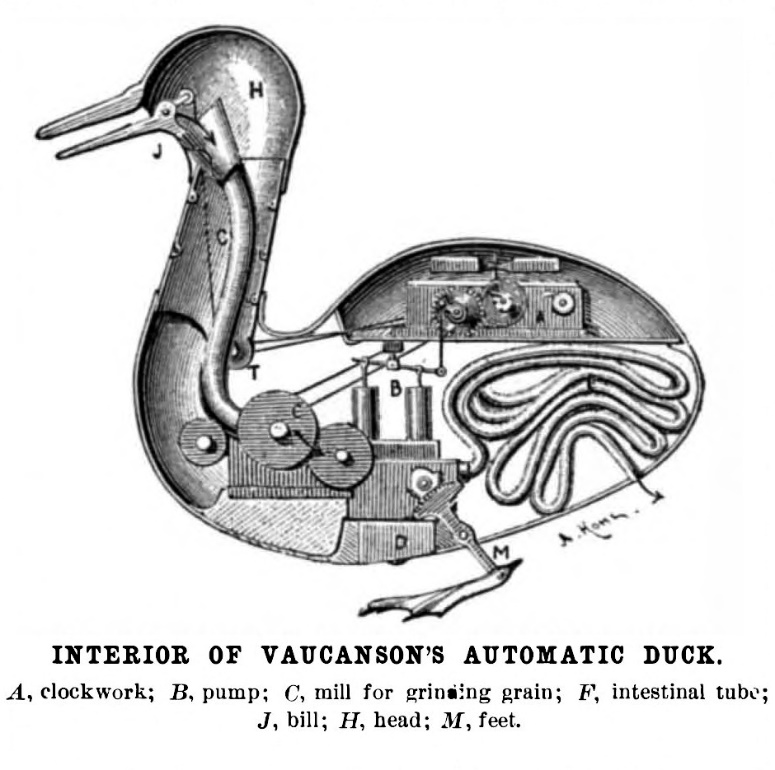
\includegraphics[width=0.97\linewidth,height=0.62\textheight,keepaspectratio]{images/intro/by_slide/s07_algunos-automatas-historicos_img01.jpeg}
    \end{column}
  \end{columns}
\end{frame}

% Página original 8
\begin{frame}{Algunos autómatas históricos}
  \small
  \begin{columns}[T,onlytextwidth]
    \begin{column}{0.62\textwidth}

        \begin{itemize}
          \item Escriba, organista y dibujante
          \begin{itemize}
            \item 1770-72-73, Jaquet-Droz
            \item Operados por mecanismos de relojería (cadenas y levas)
            \item El escriba podía mojar la pluma y escribir hasta 40 palabras.
            \item El dibujante podía realizar dibujos de Luis XV y similares, por ejemplo, una batalla naval.
            \item La organista tocaba realmente el órgano, moviendo brazos y manos
          \end{itemize}
        \end{itemize}
    \end{column}
    \begin{column}{0.38\textwidth}
      \centering
      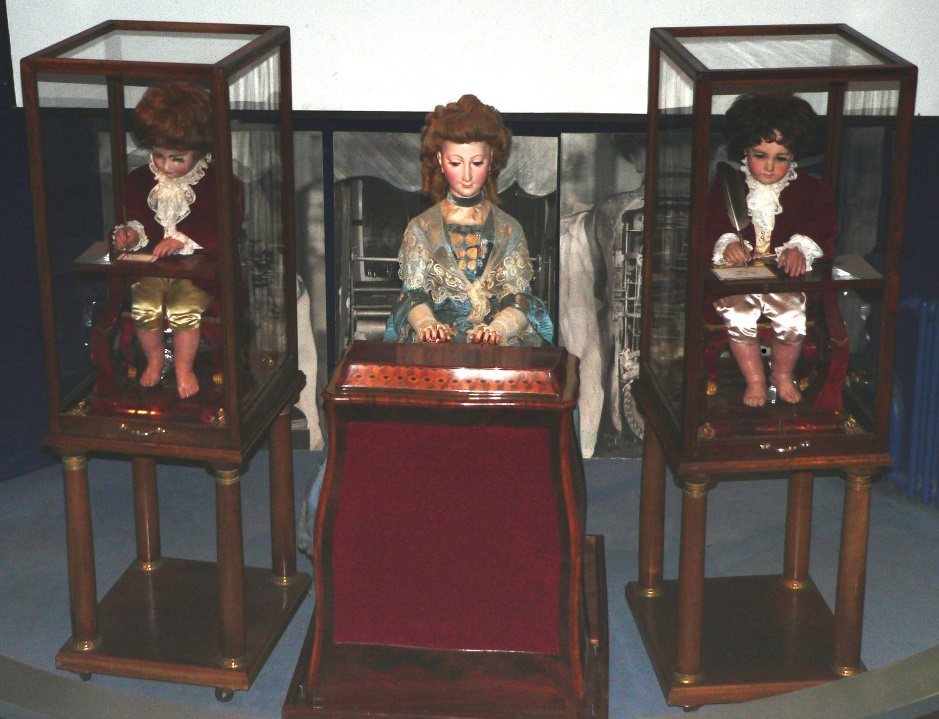
\includegraphics[width=0.97\linewidth,height=0.62\textheight,keepaspectratio]{images/intro/by_slide/s08_algunos-automatas-historicos_img01.jpeg}
    \end{column}
  \end{columns}
\end{frame}

% Página original 9
\begin{frame}{Algunos autómatas históricos}
  \small
  \begin{columns}[T,onlytextwidth]
    \begin{column}{0.62\textwidth}

        \begin{itemize}
          \item Ajedrecista
          \begin{itemize}
            \item 1769, Wolfgang von Kempelen
            \item Capaz de jugar partidas de ajedrez contra un oponente humano
            \item Movía las piezas sobre el tablero
            % \item Vídeo
          \end{itemize}
        \end{itemize}
    \end{column}
    \begin{column}{0.38\textwidth}
      \centering
      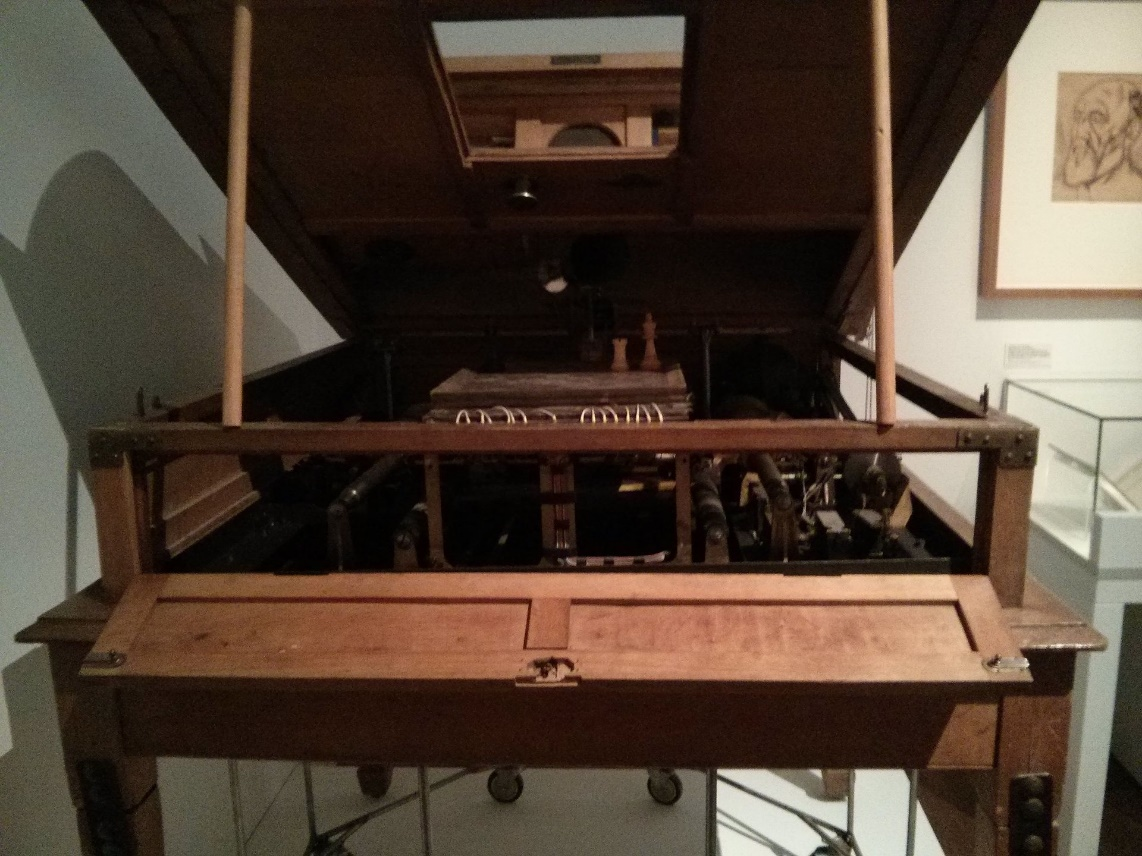
\includegraphics[width=0.97\linewidth,height=0.62\textheight,keepaspectratio]{images/intro/by_slide/s09_algunos-automatas-historicos_img01.jpeg}
    \end{column}
  \end{columns}
\end{frame}

% Página original 10
\begin{frame}{Algunos autómatas históricos}
  \small
      \centering
      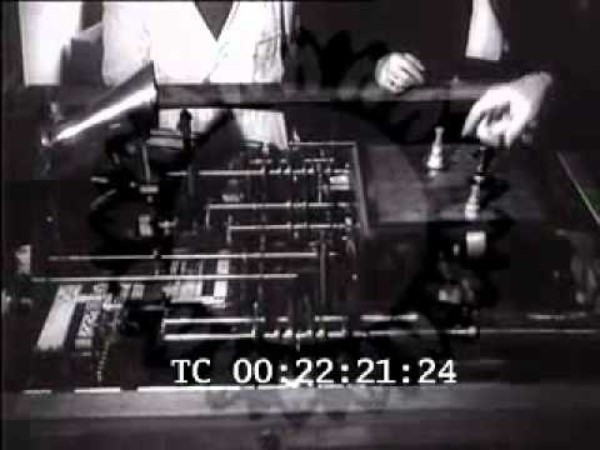
\includegraphics[width=0.97\linewidth,height=0.62\textheight,keepaspectratio]{images/intro/by_slide/s10_algunos-automatas-historicos_img01.jpeg}
\end{frame}

% Página original 11
\begin{frame}{¡Pero también hay fraudes!}
  \small
  \begin{columns}[T,onlytextwidth]
    \begin{column}{0.62\textwidth}

        \begin{itemize}
          \item Década de 1770, Wolfgang von Kempelen
          \item Hombre mecánico vestido con túnica y turbante sentado delante de un ajedrez -> ‘El Turco’
          \item von Kempelen, antes de su demostración mostró los engranajes internos del dispositivo
          \item ¡’El Turco’ era capaz de reaccionar con habilidad a las jugadas de su oponente humano!
          \item Salió de gira, y casi siempre ganaba, destruyendo la reputación de jugadores expertos
        \end{itemize}
    \end{column}
    \begin{column}{0.38\textwidth}
      \centering
      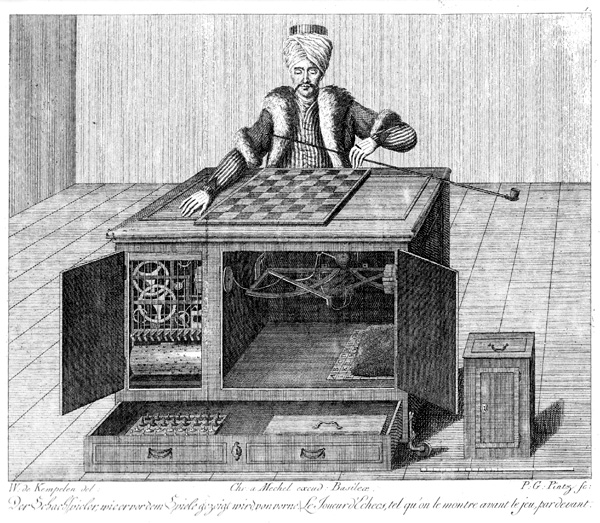
\includegraphics[width=0.97\linewidth,height=0.30\textheight,keepaspectratio]{images/intro/by_slide/s11_pero-tambien-hay-fraudes_img01.jpeg}
      \par\vspace{0.02\textheight}
      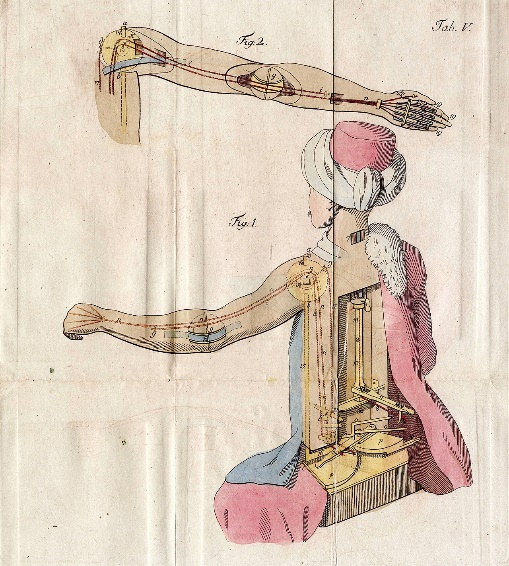
\includegraphics[width=0.97\linewidth,height=0.30\textheight,keepaspectratio]{images/intro/by_slide/s11_pero-tambien-hay-fraudes_img02.jpeg}
    \end{column}
  \end{columns}


  
\end{frame}

% Página original 12
\begin{frame}{¡Pero también hay fraudes!}
  \small
  \begin{columns}[T,onlytextwidth]
    \begin{column}{0.62\textwidth}

        \begin{itemize}
          \item Década de 1770, Wolfgang von Kempelen
          \item Hombre mecánico vestido con túnica y turbante sentado delante de un ajedrez -> ‘El Turco’
          \item von Kempelen, antes de su demostración mostró los engranajes internos del dispositivo
          \item ¡’El Turco’ era capaz de reaccionar con habilidad a las jugadas de su oponente humano!
          \item Salió de gira, y casi siempre ganaba, destruyendo la reputación de jugadores expertos
          \item Pero tenía truco…
        \end{itemize}
    \end{column}
    \begin{column}{0.38\textwidth}
      \centering
      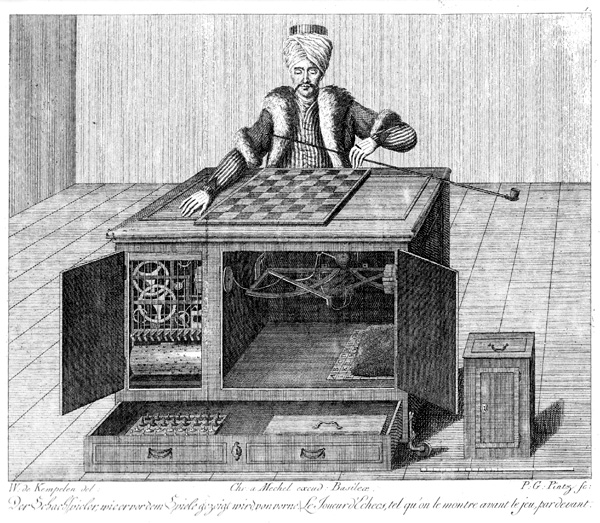
\includegraphics[width=0.97\linewidth,height=0.30\textheight,keepaspectratio]{images/intro/by_slide/s12_pero-tambien-hay-fraudes_img01.jpeg}
      \par\vspace{0.02\textheight}
      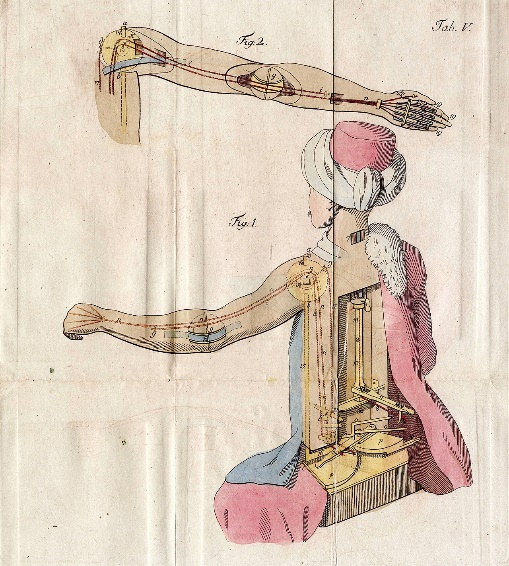
\includegraphics[width=0.97\linewidth,height=0.30\textheight,keepaspectratio]{images/intro/by_slide/s12_pero-tambien-hay-fraudes_img02.jpeg}
    \end{column}
  \end{columns}
\end{frame}

% Página original 13
\begin{frame}{Historia}
  \small
  \begin{columns}[T,onlytextwidth]
    \begin{column}{0.62\textwidth}

        \begin{itemize}
          \item Tras los autómatas, casi todos de aspecto humano, los antecesores más directos de los robots son los manipuladores teleoperados
          \item Manejo de sustancias radioactivas sin riesgo
          \item Realimentación de fuerzas para el operador
          \item En 1954, Goertz desarrolla el primer sistema de telemanipulación con servocontrol bilateral
          \item La sustitución del operador por un programa de ordenador dio paso al concepto de ‘robot’
        \end{itemize}
    \end{column}
    \begin{column}{0.38\textwidth}
      \centering
      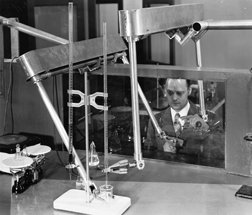
\includegraphics[width=0.97\linewidth,height=0.62\textheight,keepaspectratio]{images/intro/by_slide/s13_historia_img01.jpeg}
    \end{column}
  \end{columns}
\end{frame}

% Página original 14
\begin{frame}{Historia}
  \small
  \begin{columns}[T,onlytextwidth]
    \begin{column}{0.62\textwidth}

        \begin{itemize}
          \item Primera patente -> solicitada en 1954 por C. W. Kenward en el Reino Unido
          \item Pero fue George C. Devol (EEUU) quien estableció las bases del robot industrial moderno, Unimate, que se utilizó en la fábrica de General Motors en Trenton
          \item En 1968 se firmaron acuerdos con Kawasaki para la fabricación de robots tipo Unimate
          \item Japón aventajó en breve a EEUU gracias a Nissan
        \end{itemize}
    \end{column}
    \begin{column}{0.38\textwidth}
      \centering
      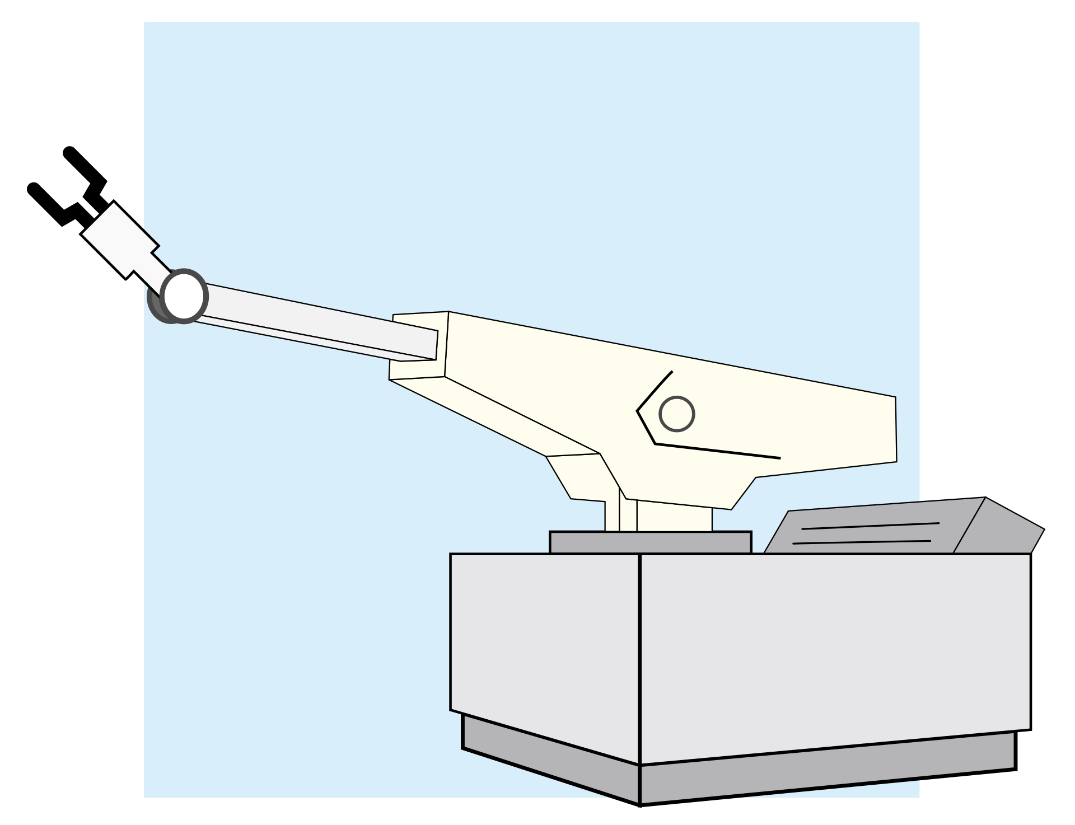
\includegraphics[width=0.97\linewidth,height=0.62\textheight,keepaspectratio]{images/intro/by_slide/s14_historia_img01.png}
    \end{column}
  \end{columns}
\end{frame}

% Página original 15
\begin{frame}{Historia}
  \small
  \begin{columns}[T,onlytextwidth]
    \begin{column}{0.62\textwidth}

        \begin{itemize}
          \item A finales de los 60, en EEUU, se proponen las bases de la investigación en robótica en las universidades:
          \begin{itemize}
            \item Inteligencia Artificial
            \item Robots móviles
            \item Bases de los manipuladores actuales (PUMA)
          \end{itemize}
          \item En Europa se comienza algo después:
          \begin{itemize}
            \item La empresa sueca ASEA crea el IRb6 en 1973
          \end{itemize}
        \end{itemize}
    \end{column}
    \begin{column}{0.38\textwidth}
      \centering
      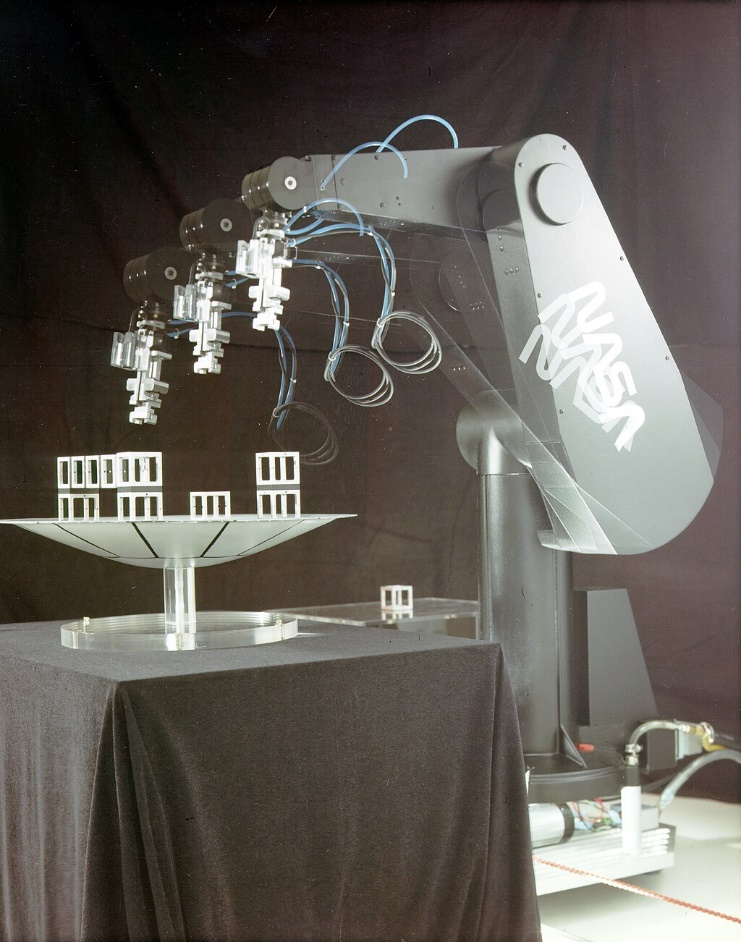
\includegraphics[width=0.97\linewidth,height=0.62\textheight,keepaspectratio]{images/intro/by_slide/s15_historia_img01.jpeg}
    \end{column}
  \end{columns}
\end{frame}

% Página original 16
\begin{frame}{Historia}
  \small
  \begin{itemize}
    \item En 1982, el prof. Makino, de la Universidad Yamanashi de Japón desarrolla el concepto de robot SCARA (Selective Compliance Assembly Robot Arm), que con pocos grados de libertad consigue ensamblar piezas
  \end{itemize}
  \vspace{0.02\textheight}
  \begin{center}
    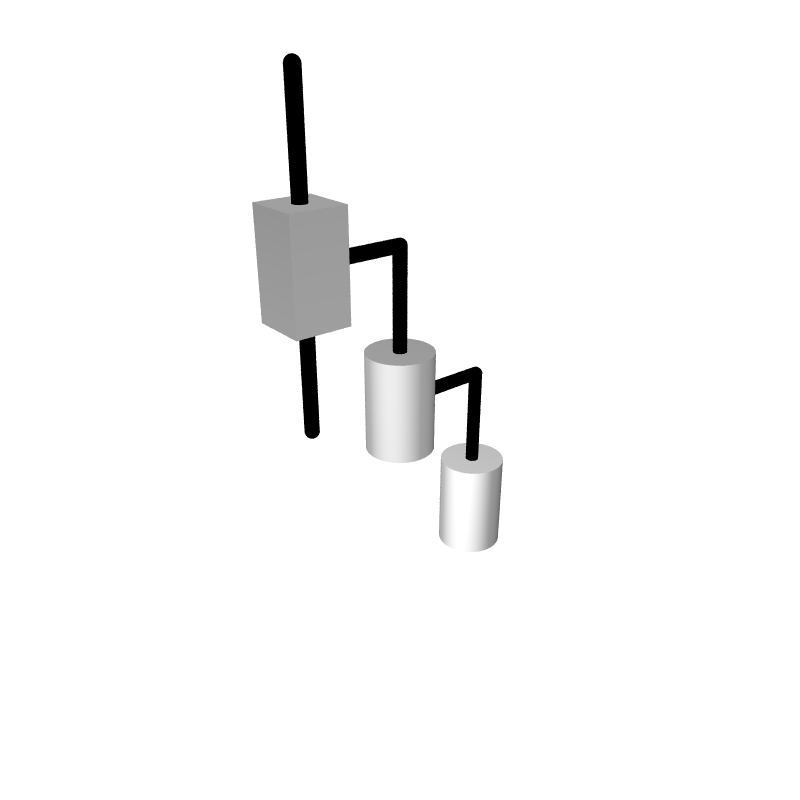
\includegraphics[width=1\linewidth,height=0.8\textheight,keepaspectratio]{images/intro/by_slide/s16_historia_img01.png}
  \end{center}
\end{frame}

% Página original 17
\begin{frame}{Historia}
  \small
  \begin{itemize}
    \item En los 70 los robots empezaron también a utilizarse en el entorno espacial y submarino
    \item En los 80 se desarrollan los primeros robots humanoides, que explota definitivamente a finales de 1996 con el lanzamiento del robot P-2, al que le siguieron otros como el ASIMO
  \end{itemize}
  \vspace{0.01\textheight}
  \begin{center}
    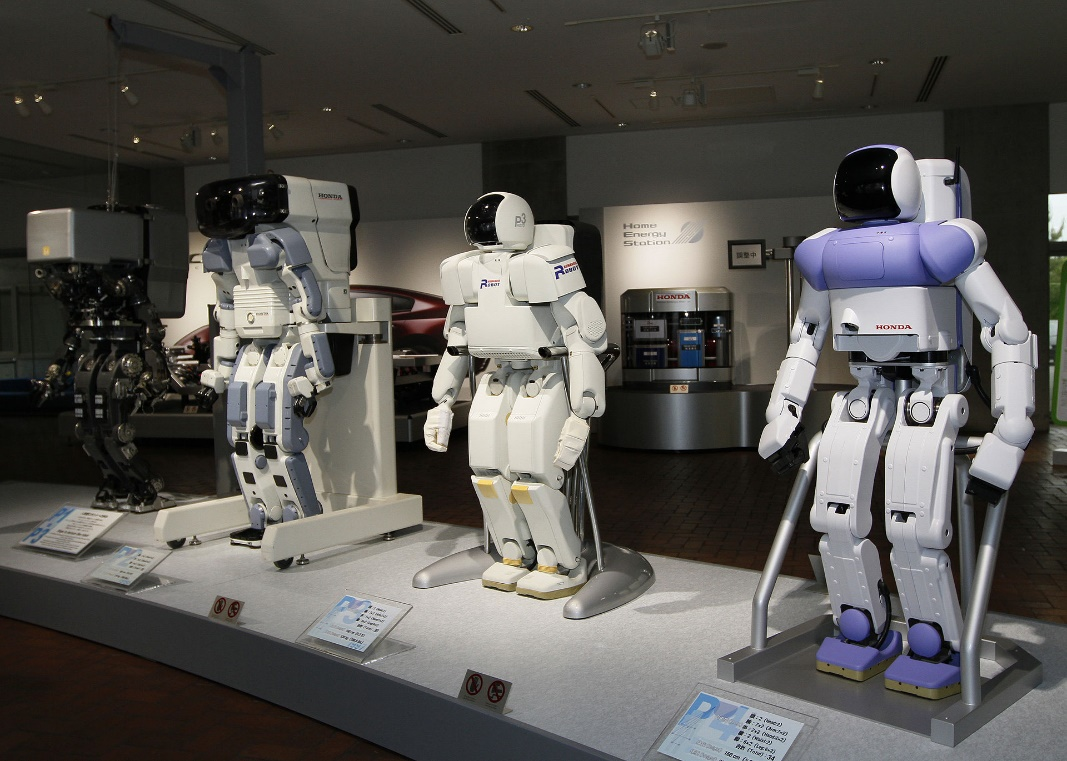
\includegraphics[width=0.47\linewidth,height=0.32\textheight,keepaspectratio]{images/intro/by_slide/s17_historia_img01.jpeg}\hspace{0.02\linewidth}
    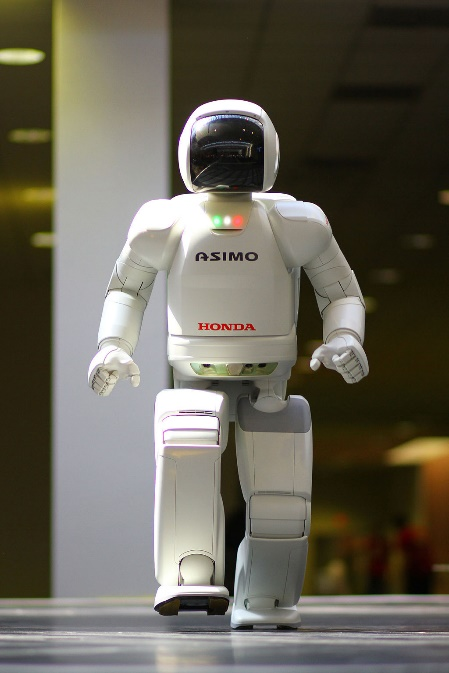
\includegraphics[width=0.47\linewidth,height=0.32\textheight,keepaspectratio]{images/intro/by_slide/s17_historia_img02.jpeg}
  \end{center}
\end{frame}

% Página original 18
\begin{frame}{Historia}
  \small
  \begin{itemize}
    \item El pionero en cuanto a robots para entretenimiento (con formas de animales) fue Sony con Aibo
  \end{itemize}
  \centering
  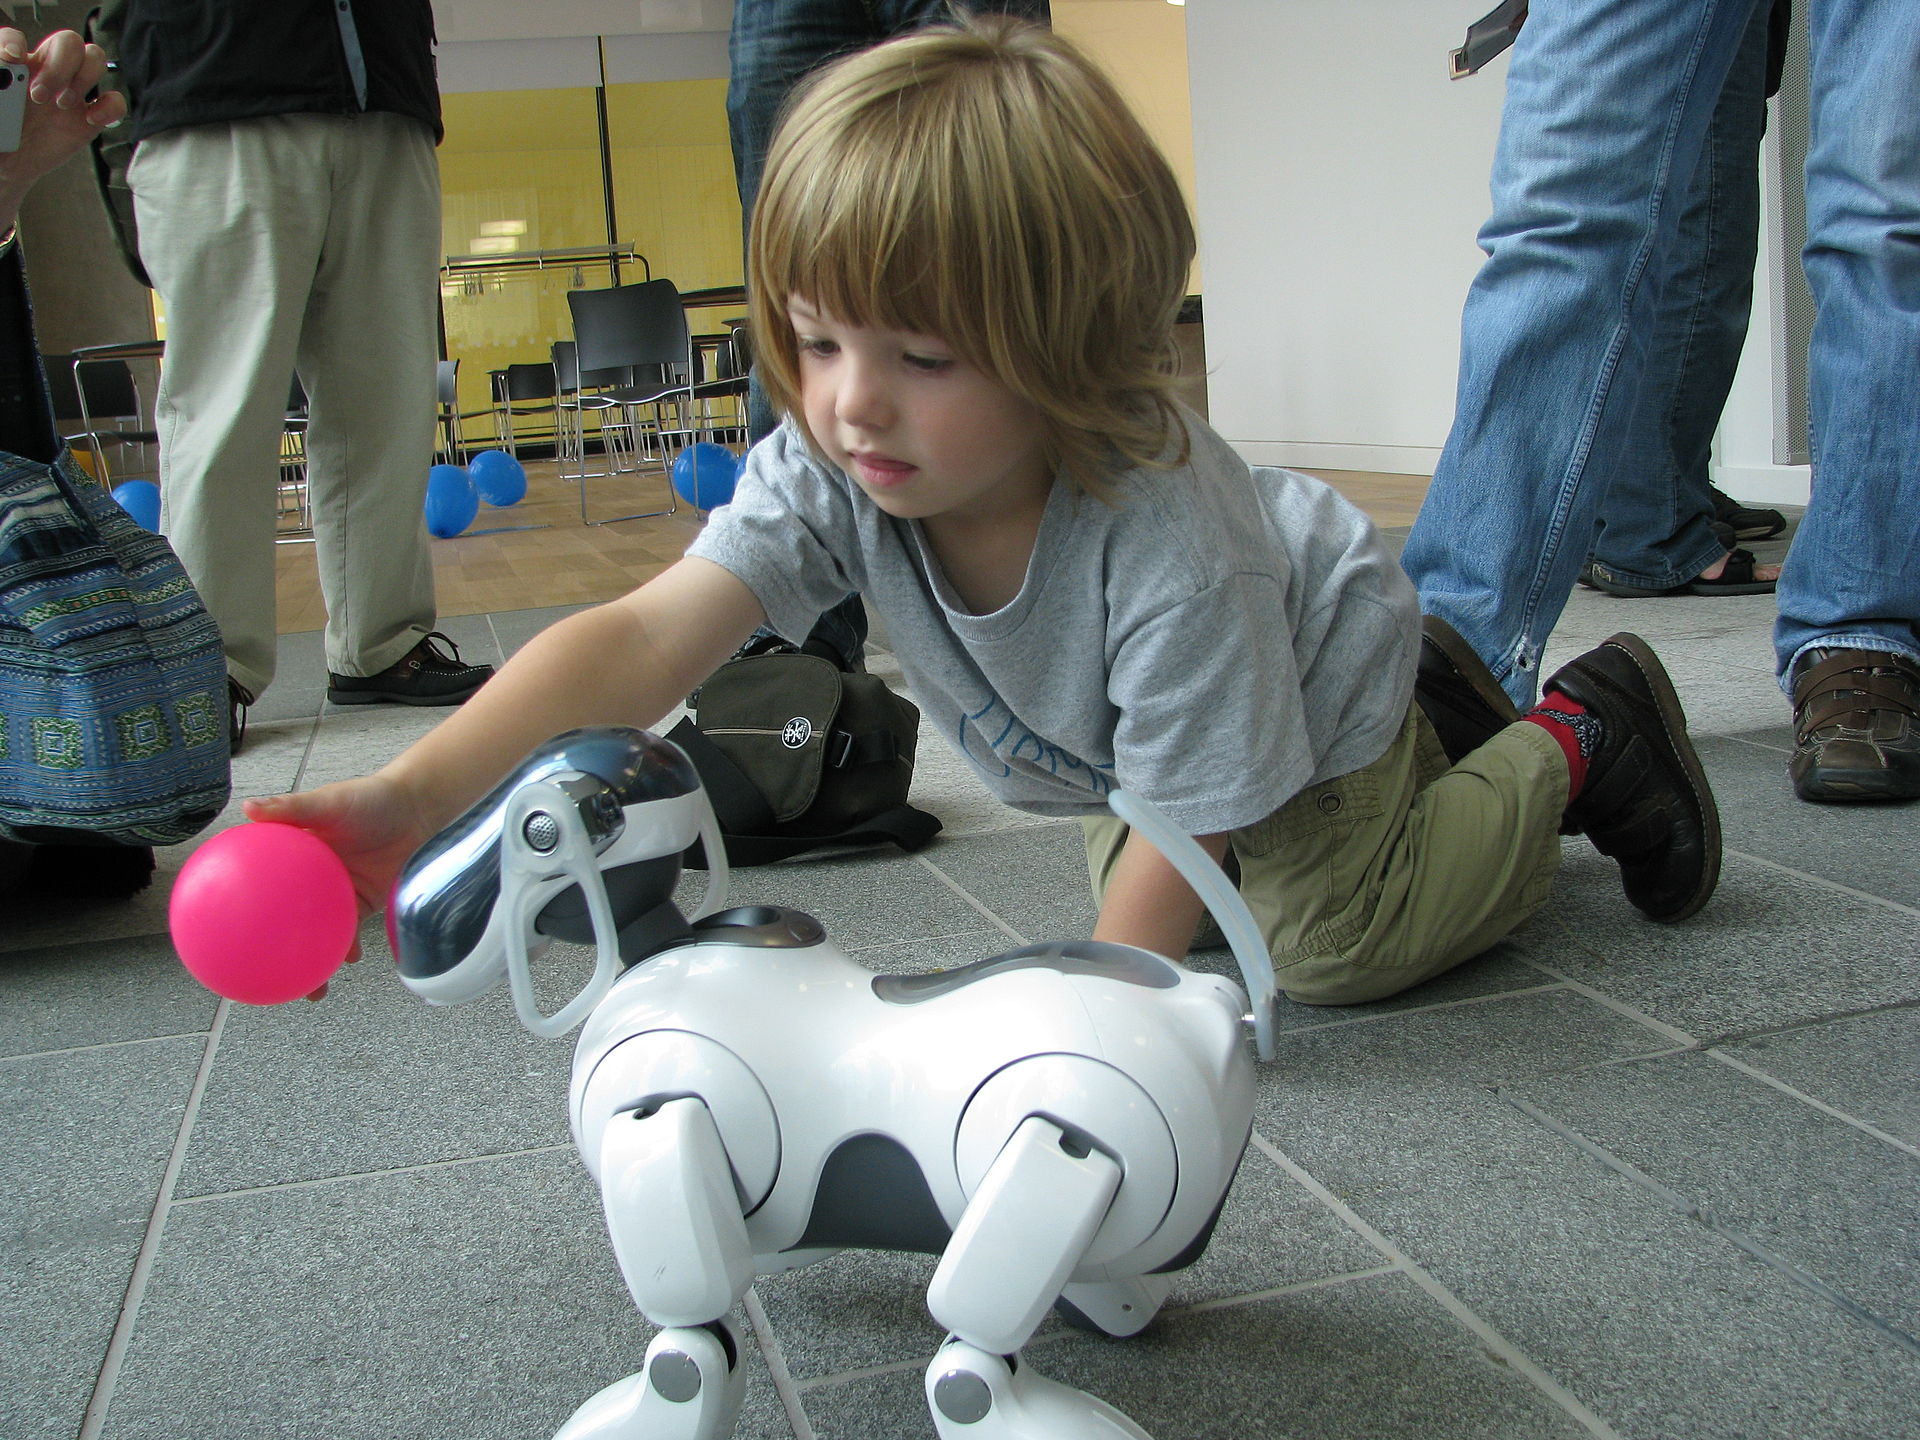
\includegraphics[width=0.97\linewidth,height=0.62\textheight,keepaspectratio]{images/intro/by_slide/s18_historia_img01.png}

\end{frame}

% Página original 19
\begin{frame}{Historia}
  \small
  \begin{itemize}
    \item Pero quien consiguió la introducción masiva de la robótica en los hogares fue iRobot en 2002
  \end{itemize}
  \centering
  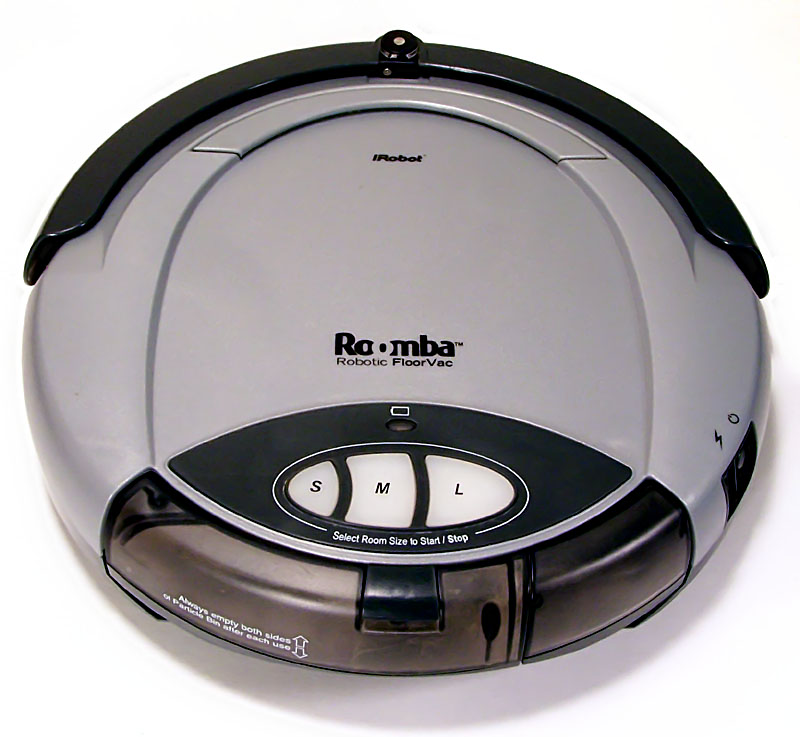
\includegraphics[width=0.97\linewidth,height=0.62\textheight,keepaspectratio]{images/intro/by_slide/s19_historia_img01.jpeg}
\end{frame}

% Página original 20
\begin{frame}{¿Qué es un robot?}
  \small
  \begin{itemize}
    \item Enciclopedia Británica:
    \begin{itemize}
      \item Máquina operada automáticamente que sustituye el esfuerzo de los humanos, aunque no tiene por qué tener apariencia humana o desarrollar sus actividades a la manera de los humanos
    \end{itemize}
    \item Merriam-Webster:
    \begin{itemize}
      \item Máquina que se asemeja a los humanos y desarrolla como ellos tareas complejas como andar o hablar
      \item Un dispositivo que desarrolla de manera automática tareas complicadas, a menudo de manera repetitiva
      \item Un mecanismo guiado por control automático
    \end{itemize}
    \item Diccionario de la Real Academia Española:
    \begin{itemize}
      \item Máquina o ingenio electrónico programable que es capaz de manipular objetos y realizar diversas operaciones
    \end{itemize}
  \end{itemize}
  % \vspace{0.01\textheight}
  % \begin{center}
  %   \includegraphics[width=0.72\linewidth,height=0.16\textheight,keepaspectratio]{images/intro/by_slide/s20_que-es-un-robot_img01.png}
  %   \par\vspace{0.01\textheight}
  %   \includegraphics[width=0.72\linewidth,height=0.16\textheight,keepaspectratio]{images/intro/by_slide/s20_que-es-un-robot_img02.png}
  %   \par\vspace{0.01\textheight}
  %   \includegraphics[width=0.72\linewidth,height=0.16\textheight,keepaspectratio]{images/intro/by_slide/s20_que-es-un-robot_img03.png}
  % \end{center}
\end{frame}

% Página original 21
\section{Definición}


% Página original 22
\begin{frame}{¿Qué es un robot?}
  \small
  \begin{columns}[c,onlytextwidth]
    \begin{column}{0.62\textwidth}
      \begin{itemize}
        \item Parece que, incluso en la actualidad, las definiciones resultan insuficientes
        \item Por ello, es común añadir un adjetivo al término ‘robot’ que permita acotar sus características o campo de actuación:
        \begin{itemize}
          \item Robot manipulador
          \item Robot de servicio
          \item Robot móvil
          \item Robot submarino
          \item Robot espacial
          \item Robot autónomo
          \item Robot humanoide
          \item ...
        \end{itemize}
      \end{itemize}
    \end{column}
    \begin{column}{0.38\textwidth}
      \centering
      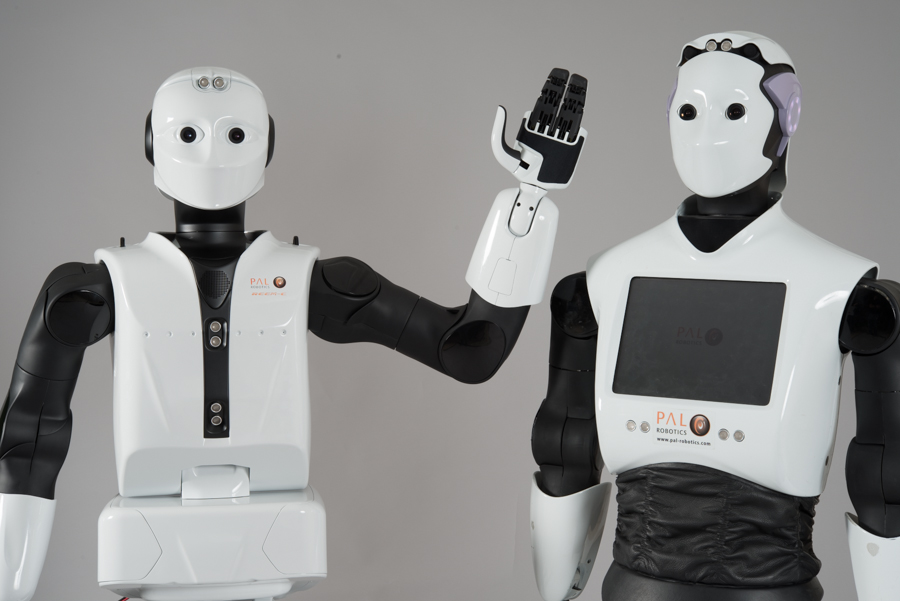
\includegraphics[width=0.97\linewidth,height=0.62\textheight,keepaspectratio]{images/intro/by_slide/s22_que-es-un-robot_img01.jpeg}
    \end{column}
  \end{columns}
\end{frame}

% Página original 23
\begin{frame}{Robots vs. profesionales de la salud}
  \small
  \begin{itemize}
    \item ¿Reemplazo o colaboración?
    \item Diferentes roles:
    \begin{itemize}
      \item Profesional $\rightarrow$ decisión, supervisión
      \item Robot $\rightarrow$ ejecución
    \end{itemize}
  \end{itemize}
  % \vspace{0.25em}
  \begin{center}
    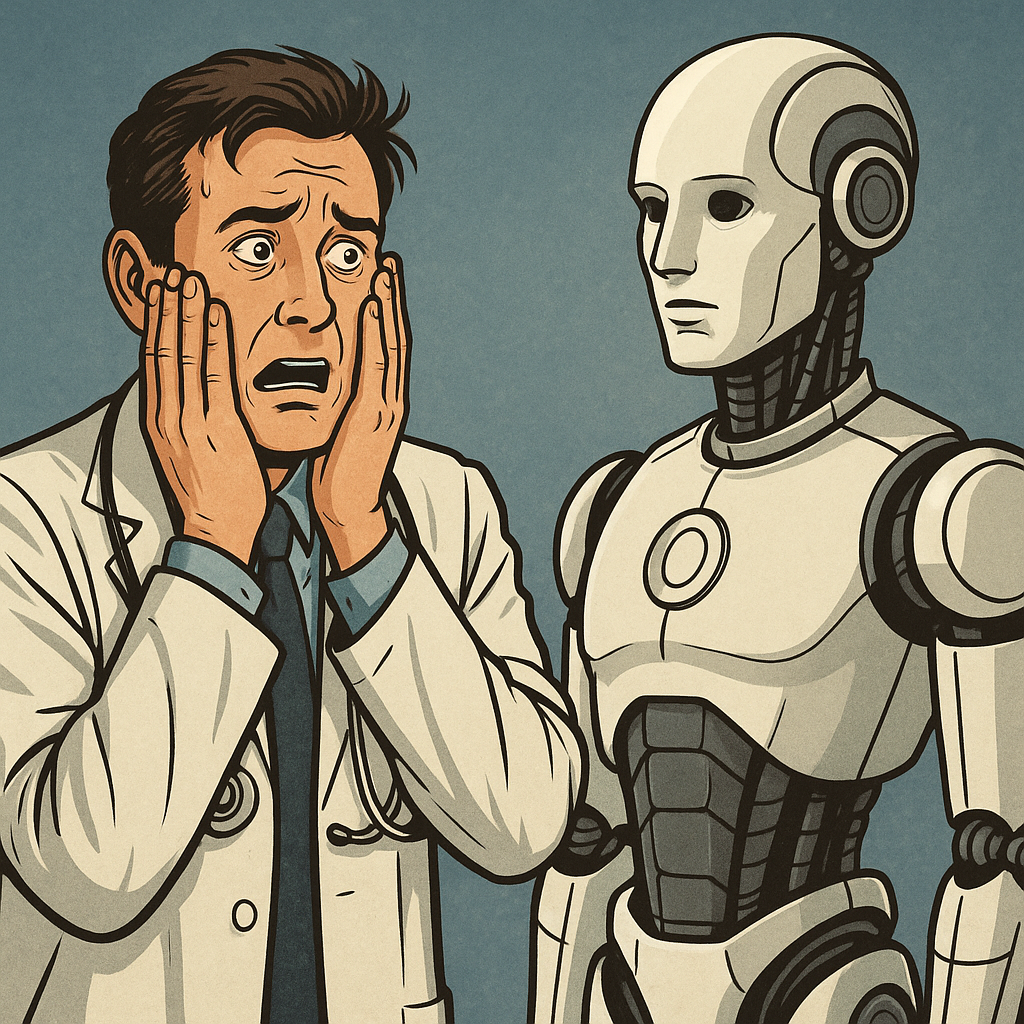
\includegraphics[width=0.78\linewidth,height=0.5\textheight,keepaspectratio]{images/intro/by_slide/s23_robots-vs-profesionales-de-la-salud_img01.png}%
    \par\vspace{0.25em}
  \end{center}
\end{frame}

% Página original 24
\section{Robótica social y asistencial}


% Página original 25
\begin{frame}{Robot social}
  \small
  \begin{itemize}
    \item Comportamientos en sociedad:
    \begin{itemize}
      \item Reglas sociales
      \item Roles en grupos
    \end{itemize}
    \item Robots autónomos con capacidades de conexión y comunicación con humanos y otros robots sociales
    \item Algunas aplicaciones: compañía, terapia, educación
  \end{itemize}
  \vspace{0.25em}
  \begin{center}
    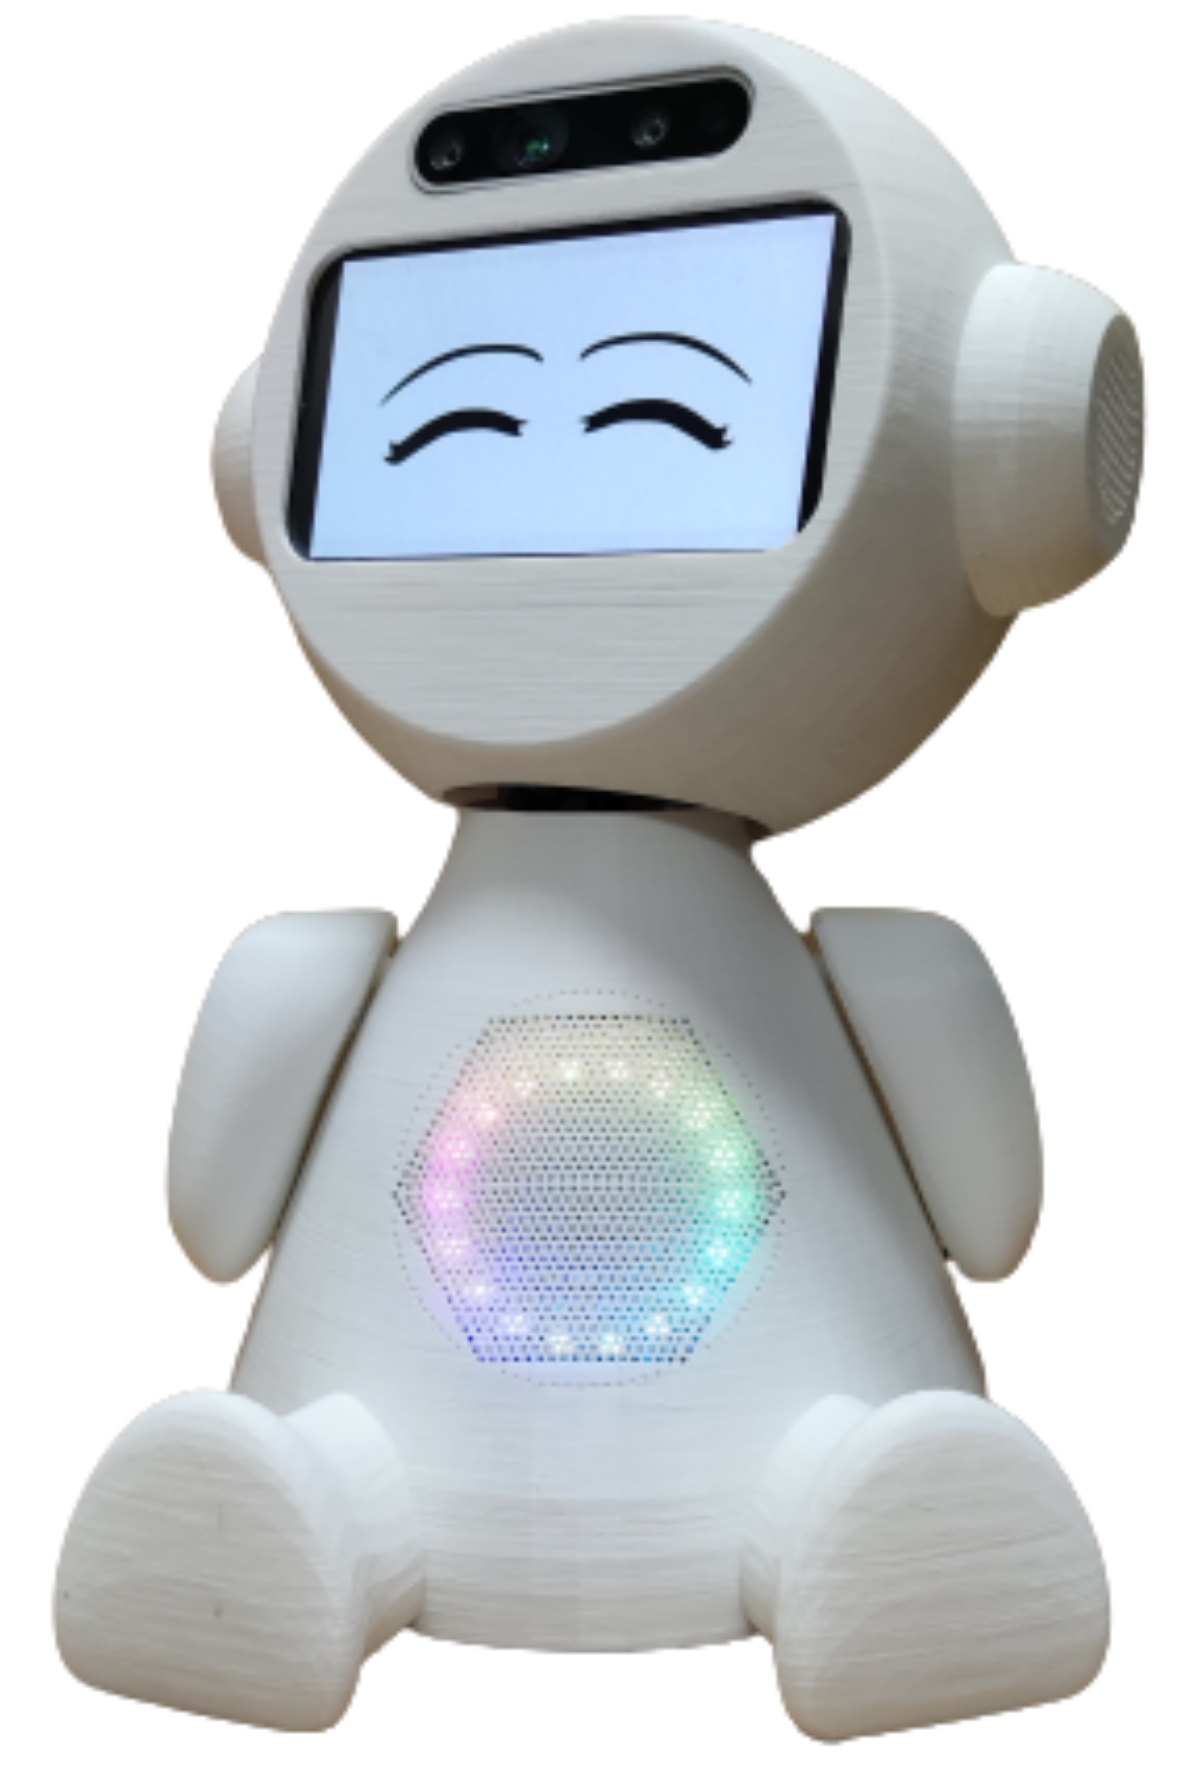
\includegraphics[width=0.78\linewidth,height=0.36\textheight,keepaspectratio]{images/intro/by_slide/s25_robot-social_img01.png}%
    \par\vspace{0.25em}
  \end{center}
\end{frame}

% Página original 26
\begin{frame}{Robot social}
  \small  
  \begin{itemize}
    \item Se compone de:
    \begin{itemize}
      \item Sensores
      \item Actuadores
      \item Computadores
    \end{itemize}
    \item Hay que programarlo para que funcione $\rightarrow$ inteligencia
  \end{itemize}
  \begin{center}
    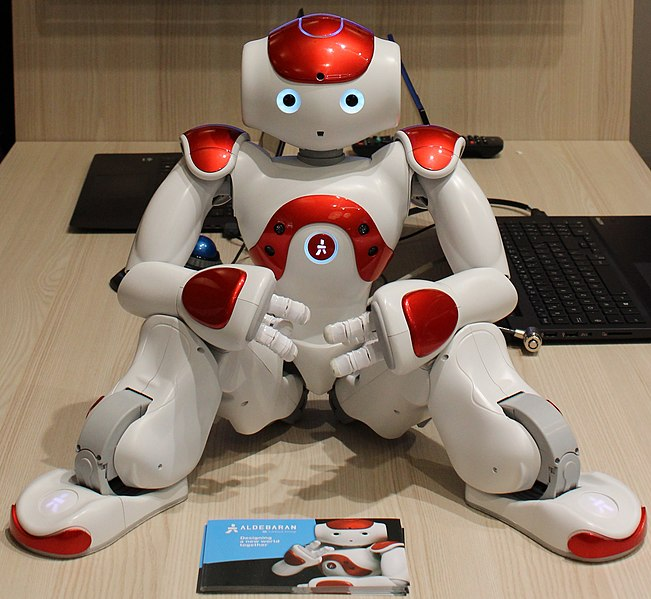
\includegraphics[width=0.78\linewidth,height=0.5\textheight,keepaspectratio]{images/intro/by_slide/s26_robot-social_img01.jpeg}%
    \par\vspace{0.25em}
  \end{center}
\end{frame}

% Página original 27
% \begin{frame}{Sensores y actuadores}
%   \small
%   \vspace{0.25em}
%   \begin{center}
%     \includegraphics[width=0.48\linewidth,height=0.27\textheight,keepaspectratio]{images/intro/by_slide/s27_sensores-y-actuadores_img01.png}%
%     \hfill
%     \includegraphics[width=0.48\linewidth,height=0.27\textheight,keepaspectratio]{images/intro/by_slide/s27_sensores-y-actuadores_img02.jpeg}%
%     \par\vspace{0.25em}
%   \end{center}
%   \begin{itemize}
%     \item •… Picture by Kelly
%   \end{itemize}
%   \begin{itemize}
%     \item Sensores:
%     \item Cámaras
%     \item US
%     \item LiDAR
%     \item Encoders •…
%     \item Actuadores:
%     \item Motores eléctricos
%     \item Sistemas de locomoción
%     \item Sistemas de manipulación
%   \end{itemize}
% \end{frame}

% % Página original 28
% \begin{frame}{Sensores y actuadores}
%   \small
%   \begin{itemize}
%     \item Sensores:
%     \item Miden magnitudes físicas del entorno del robot (distancia, luz, etc.)
%     \item Permiten conocer tanto el estado del robot como el mundo que le rodea
%     \item El tipo de sensores utilizados depende de la tarea a realizar
%     \item Actuadores:
%     \item Elementos mediante los cuales el robot interactúa con el mundo
%     \item Le dotan de capacidades (movimiento, etc.)
%     \item En general (mucho), dividen a la robótica en:
%     \item Robots móviles
%     \item Robots manipuladores
%   \end{itemize}
% \end{frame}

% % Página original 29
% \begin{frame}{Computadores}
%   \small
%   \vspace{0.25em}
%   \begin{center}
%     \includegraphics[width=0.78\linewidth,height=0.36\textheight,keepaspectratio]{images/intro/by_slide/s29_computadores_img01.jpeg}%
%     \par\vspace{0.25em}
%   \end{center}
%   \begin{itemize}
%     \item Ordenadores
%     \item Microprocesadores
%     \item Microcontroladores
%   \end{itemize}
% \end{frame}

% Página original 30
\begin{frame}{Ejemplo: Myon}
  \small
  \begin{columns}[c,onlytextwidth]
    \begin{column}{0.48\textwidth}
      \begin{itemize}
        \item Humanoide con forma de niño
        \item Práctica diaria de interacciónes sociales - Canto - Baile - Juegos
      \end{itemize}
    \end{column}
    \begin{column}{0.52\textwidth}
      \centering
      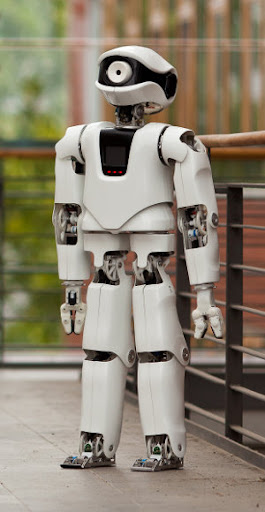
\includegraphics[width=0.97\linewidth,height=0.62\textheight,keepaspectratio]{images/intro/by_slide/s30_ejemplo-myon_img01.png}
    \end{column}
  \end{columns}
\end{frame}

% Página original 31
\begin{frame}{Ejemplo: Robear}
  \small
  \begin{columns}[c,onlytextwidth]
    \begin{column}{0.48\textwidth}
      \begin{itemize}
        \item Robot enfermero
        \item Transporte de personas
      \end{itemize}
    \end{column}
    \begin{column}{0.52\textwidth}
      \centering
      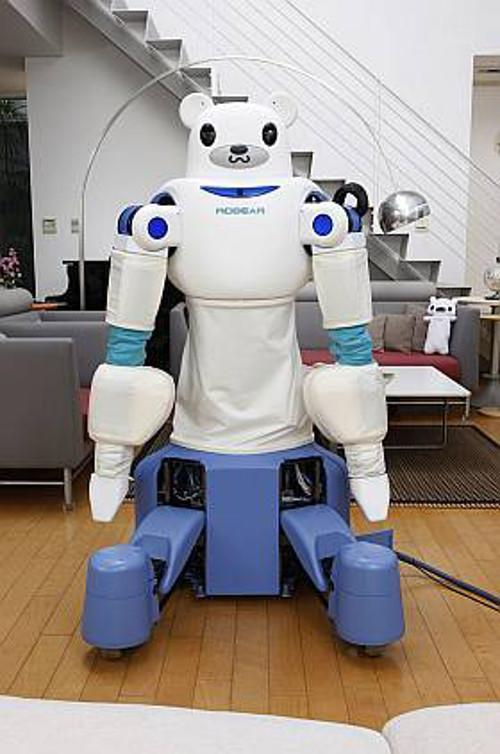
\includegraphics[width=0.97\linewidth,height=0.62\textheight,keepaspectratio]{images/intro/by_slide/s31_ejemplo-robear_img01.png}
    \end{column}
  \end{columns}
\end{frame}

% Página original 32
\begin{frame}{Ejemplo: Pepper}
  \small
  \begin{columns}[c,onlytextwidth]
    \begin{column}{0.48\textwidth}
      \begin{itemize}
        \item Interacción emocional
        \item Expresiones faciales
        \item Gestos
        \item Tono de voz
      \end{itemize}
    \end{column}
    \begin{column}{0.52\textwidth}
      \centering
      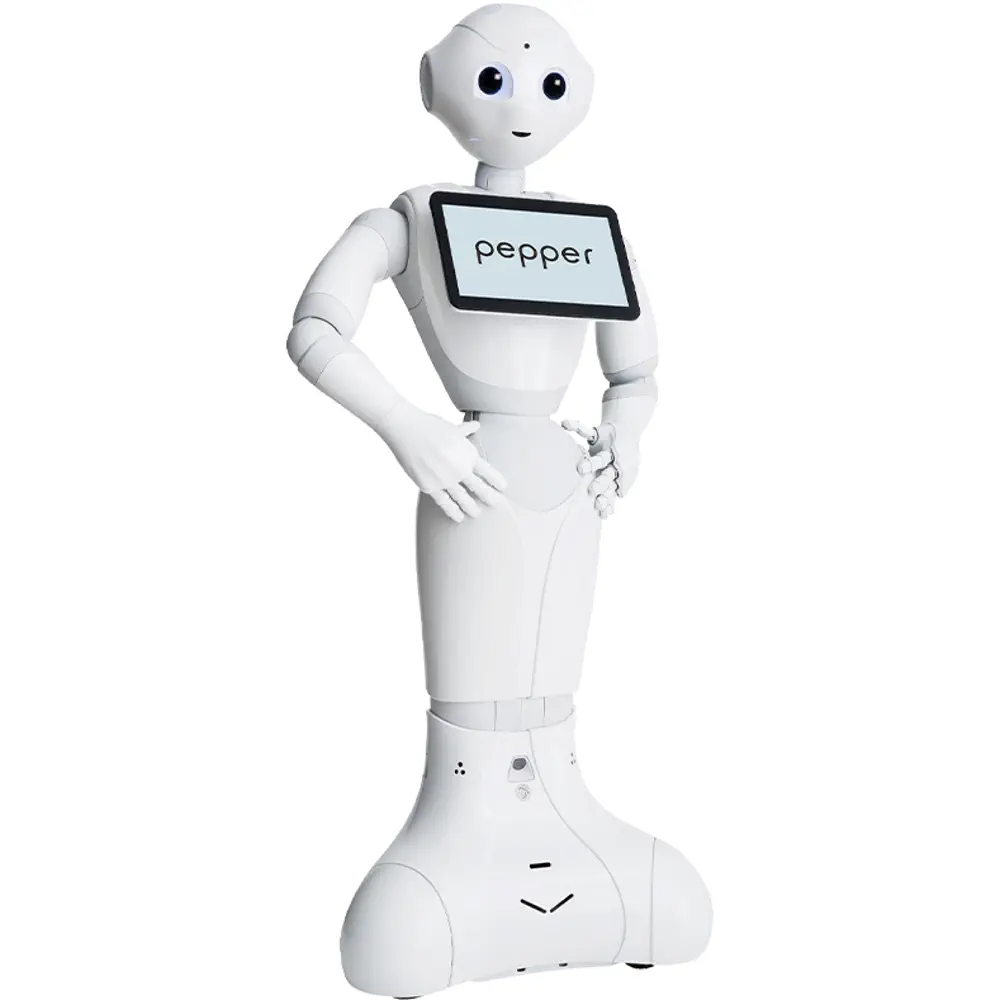
\includegraphics[width=0.97\linewidth,height=0.62\textheight,keepaspectratio]{images/intro/by_slide/s32_ejemplo-pepper_img01.png}
    \end{column}
  \end{columns}
\end{frame}

% Página original 33
\begin{frame}{Ejemplo: PARO y Aibo}
  \small
  \begin{itemize}
    \item Interacciones sociales (soledad)
    \item Actividades interactivas
  \end{itemize}
  % \vspace{0.25em}
  \begin{center}
    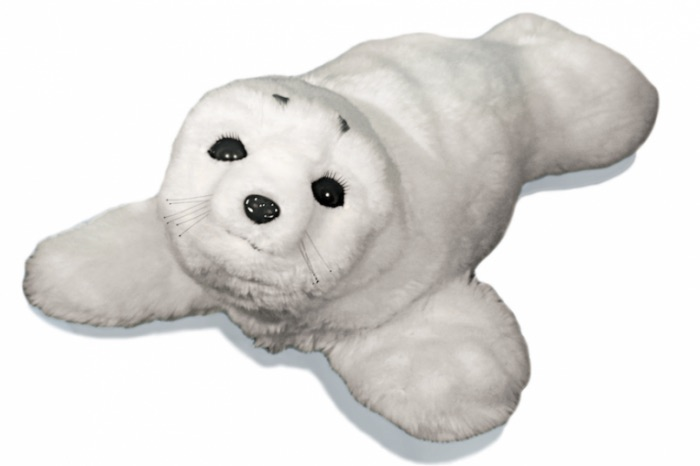
\includegraphics[width=0.47\linewidth,height=0.5\textheight,keepaspectratio]{images/intro/by_slide/s33_ejemplo-paro-y-aibo_img01.png}%
    \hspace{0.01\linewidth}
    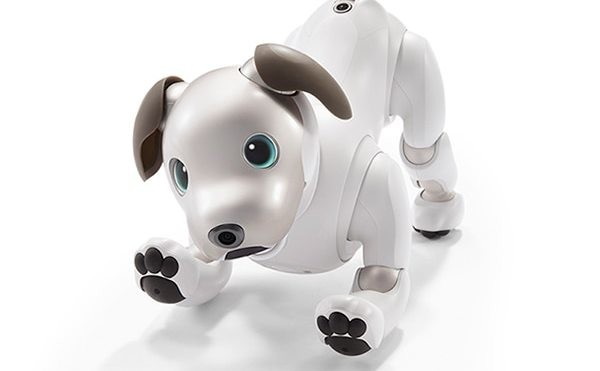
\includegraphics[width=0.47\linewidth,height=0.5\textheight,keepaspectratio]{images/intro/by_slide/s33_ejemplo-paro-y-aibo_img02.png}%
    \par\vspace{0.25em}
  \end{center}
\end{frame}

% Página original 34
\begin{frame}{Paradigma de arquitectura}
  \small
  \vspace{0.25em}
  \begin{center}
    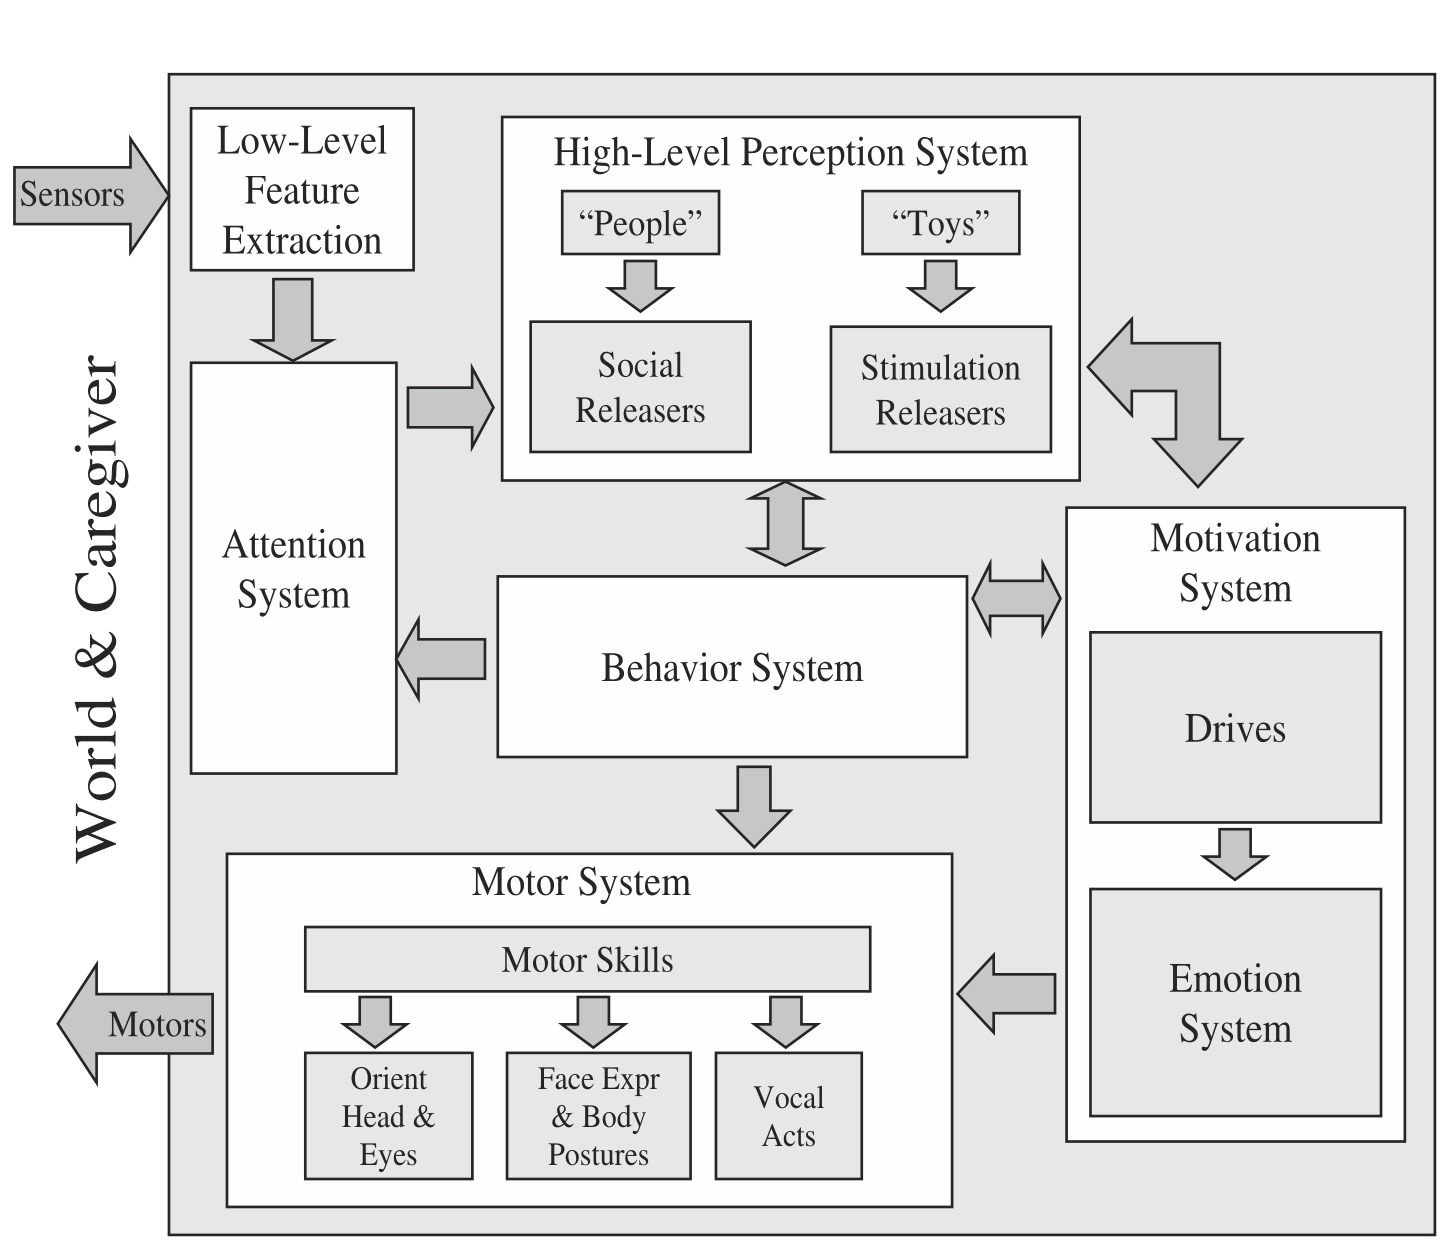
\includegraphics[width=1\linewidth,height=0.8\textheight,keepaspectratio]{images/intro/by_slide/s34_paradigma-de-arquitectura_img01.png}%
    \par\vspace{0.25em}
  \end{center}
  \vfill
\end{frame}


% Página original 36
\begin{frame}{Arquitectura software}
  \small
  % \vspace{0.25em}
  \begin{center}
    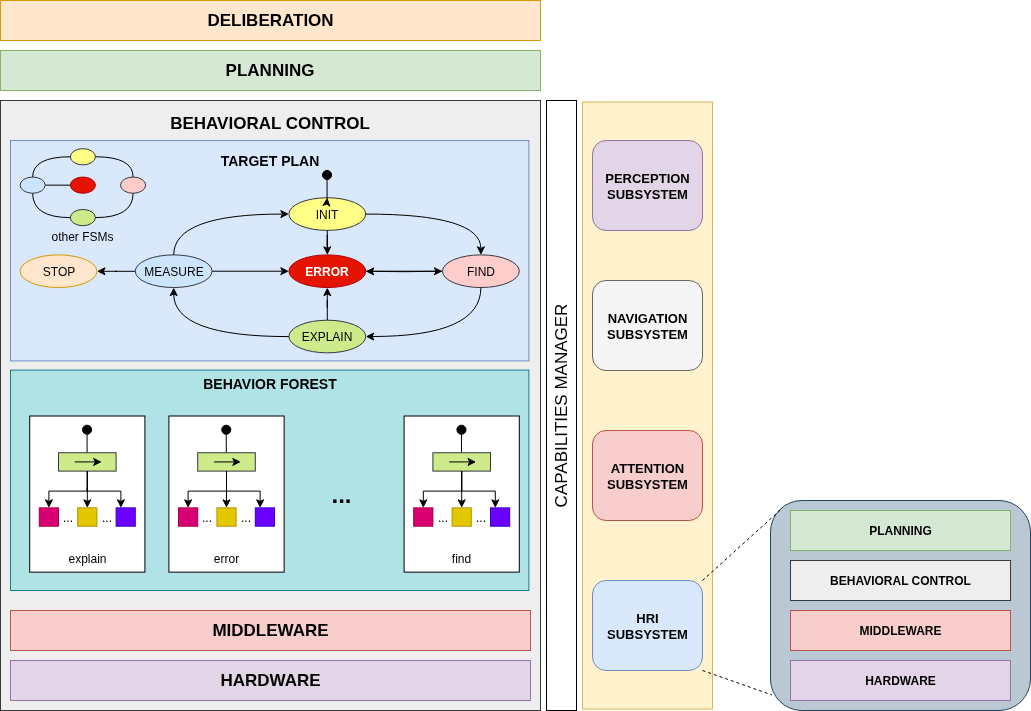
\includegraphics[width=1\linewidth,height=.85\textheight,keepaspectratio]{images/intro/by_slide/s36_arquitectura-software_img01.png}%
    % \par\vspace{0.25em}
  \end{center}
  \vfill
\end{frame}

% Página original 37
\section{Robótica y discapacidad intelectual}


% Página original 38
\begin{frame}{Discapacidad intelectual}
  \small
  \begin{columns}[c,onlytextwidth]
    \begin{column}{0.62\textwidth}
      \begin{itemize}
        \item Condición del neurodesarrollo con limitaciones en el funcionamiento intelectual y la conducta adaptativa
        \item Afecta habilidades sociales, prácticas y conceptuales
        \item Necesita apoyos personalizados durante toda la vida
        \item Robots socialmente asistivos:
        \begin{itemize}
          \item Diseñados para ayudar en la terapia e interacción social
          \item No realizan tareas físicas, sino motivacionales y educativas
        \end{itemize}
      \end{itemize}
    \end{column}
    \begin{column}{0.38\textwidth}
      \centering
      
\includegraphics[width=0.97\linewidth,height=0.62\textheight,keepaspectratio]{images/intro/by_slide/s38_discapacidad-intelectual_img01.png}
    \end{column}
  \end{columns}
\end{frame}

% Página original 39
\begin{frame}{Diversas aplicaciones}
  \small
  \begin{itemize}
    \item Intervención con niños con TEA y DI mediante robots humanoides
    \item Enseñanza de habilidades sociales: turno, imitación, atención conjunta
    \item Intervenciones conductuales personalizadas con robots socialmente asistivos
    \item Beneficios observados:
    \begin{itemize}
      \item Aumento del enfoque y la atención
      \item Mejora en la comunicación y la interacción
      \item Los robots se perciben como no amenazantes, facilitando la relación
    \end{itemize}
  \end{itemize}
\end{frame}

% Página original 40
\begin{frame}{Inclusión educativa}
  \small
  \begin{itemize}
    \item Asistencia al aula de manera remota mediado por robot:
    \begin{itemize}
      \item ¿Cómo tiene que ser el robot físicamente (apariencia, tamaño, etc.)?
    \end{itemize}
    \item Intervenciones dirigidas a la mejora de\footnote{Parra, J. R. (2021). Robótica para la inclusióneducativa: una revisión sistemática. RiiTE Revista interuniversitaria de investigación en Tecnología Educativa, 150-171}:
    \begin{itemize}
      \item ¿Cómo tiene que ser el robot físicamente (apariencia, tamaño, etc.)?
      \item Habilidades sociales y trabajo en equipo inclusión educativa: una revisión sistemática. RiiTE Revista interuniversitaria
      \item Atención y concentración
      \item Agresividad (disminución) y aceptación de la frustración -Habla
      \item Motricidad fina y coordinación óculo-manual -Autoestima
    \end{itemize}
  \end{itemize}
\end{frame}

% Página original 41
\begin{frame}{Limitaciones y retos}
  \small
  \begin{itemize}
    \item Falta de evidencia empírica sólida a largo plazo
    \item Riesgo de reemplazar la interacción humana
    \item Necesidad de acompañamiento profesional constante
  \end{itemize}
  \begin{center}
    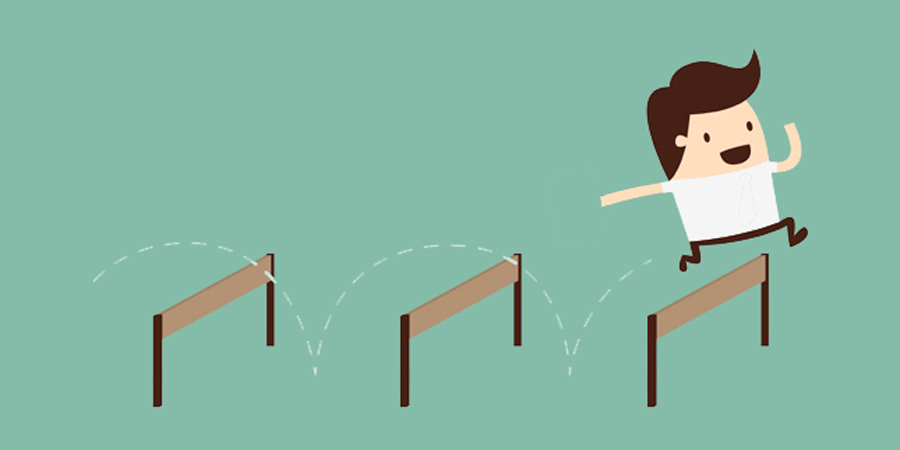
\includegraphics[width=0.78\linewidth,height=0.36\textheight,keepaspectratio]{images/intro/by_slide/s41_limitaciones-y-retos_img01.png}%
    \par\vspace{0.25em}
  \end{center}
\end{frame}

% Página original 42
\section{Robótica y personas mayores}

% Página original 43
\begin{frame}{Envejecimiento poblacional}
  \small 
  \begin{itemize}
    \item Crecimiento y envejecimiento de la población:
    \begin{itemize}
      \item 10\% de personas mayores en el año 2000
      \item 24\% en el 2030
      \item Aumento de la esperanza de vida $\rightarrow$ necesidad de más cuidadores
    \end{itemize}
    \item Tendencia \textit{ageing in place} $\rightarrow$ mantener a las personas mayores en sus hogares el mayor tiempo posible
  \end{itemize}
  \begin{center}
    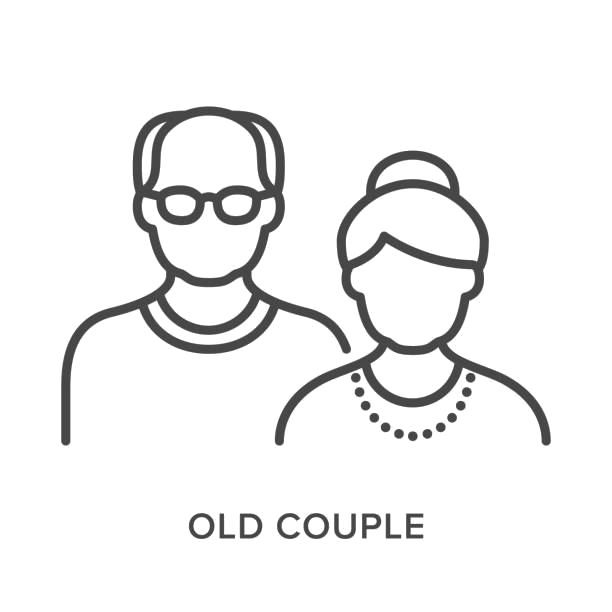
\includegraphics[width=0.78\linewidth,height=0.5\textheight,keepaspectratio]{images/intro/by_slide/s43_envejecimiento-poblacional_img01.png}%
    \par\vspace{0.25em}
  \end{center}
\end{frame}

% Página original 44
\begin{frame}{Áreas de aplicación principales}
  \small
  \begin{columns}[c,onlytextwidth]
    \begin{column}{0.62\textwidth}
      \begin{itemize}
        \item Aislamiento social
        \item Personas dependientes
        \item Deterioro cognitivo
        \item Problemas de movilidad
        \item Monitorización
        \item Recreación
        \item Recordatorios
        \item Detección de caídas
        \item Tareas domésticas
        \item …
      \end{itemize}
    \end{column}
    \begin{column}{0.38\textwidth}
      \centering
      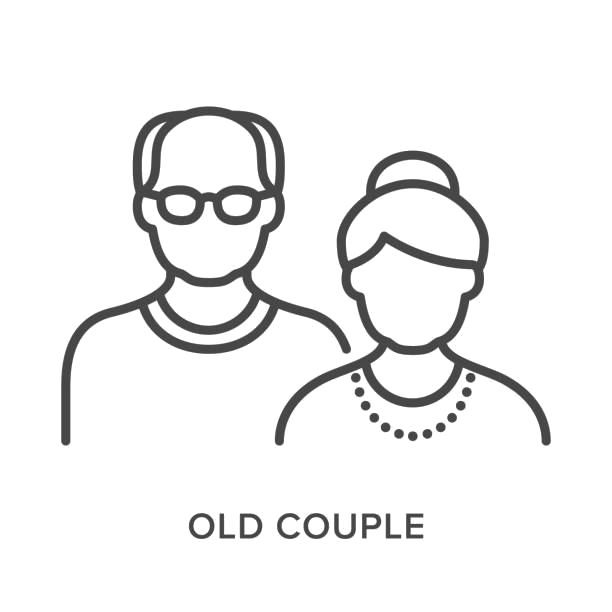
\includegraphics[width=0.97\linewidth,height=0.62\textheight,keepaspectratio]{images/intro/by_slide/s44_areas-de-aplicacion-principales_img01.png}
    \end{column}
  \end{columns}
\end{frame}

% Página original 45
\begin{frame}{Robots de compañía}
  \small
  \vspace{0.15em}
  \begin{center}
    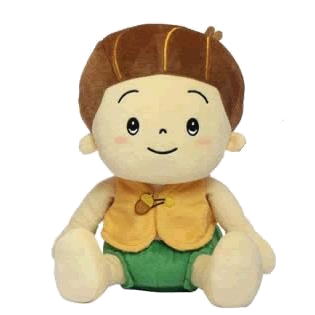
\includegraphics[width=0.235\linewidth,height=0.13\textheight,keepaspectratio]{images/intro/by_slide/s45_robots-de-compania_img01.jpeg}%
    \hspace{0.008\linewidth}
    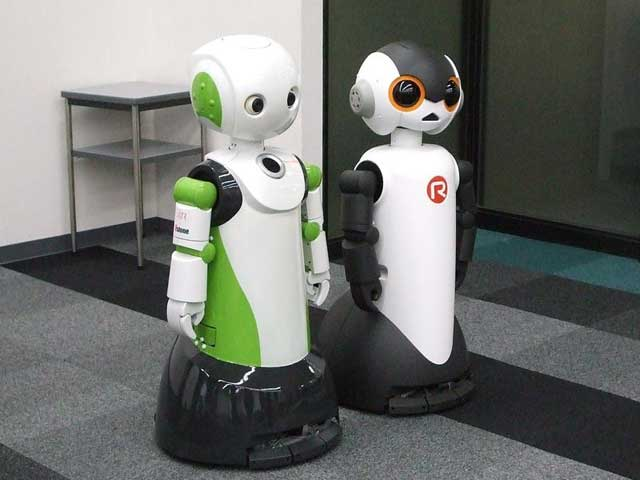
\includegraphics[width=0.235\linewidth,height=0.13\textheight,keepaspectratio]{images/intro/by_slide/s45_robots-de-compania_img02.jpeg}%
    \hspace{0.008\linewidth}
    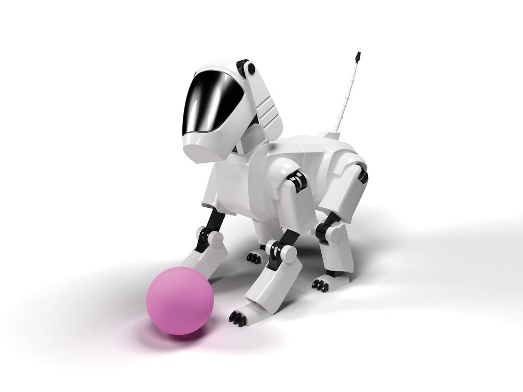
\includegraphics[width=0.235\linewidth,height=0.13\textheight,keepaspectratio]{images/intro/by_slide/s45_robots-de-compania_img03.jpeg}%
    \hspace{0.008\linewidth}
    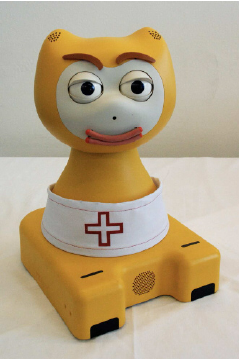
\includegraphics[width=0.235\linewidth,height=0.13\textheight,keepaspectratio]{images/intro/by_slide/s45_robots-de-compania_img04.png}%
    \par\vspace{0.18em}

    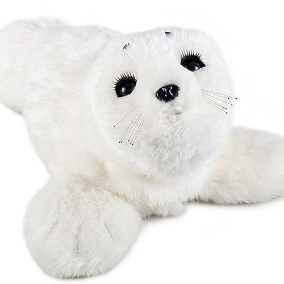
\includegraphics[width=0.235\linewidth,height=0.13\textheight,keepaspectratio]{images/intro/by_slide/s45_robots-de-compania_img05.png}%
    \hspace{0.008\linewidth}
    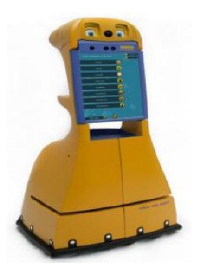
\includegraphics[width=0.235\linewidth,height=0.13\textheight,keepaspectratio]{images/intro/by_slide/s45_robots-de-compania_img06.png}%
    \hspace{0.008\linewidth}
    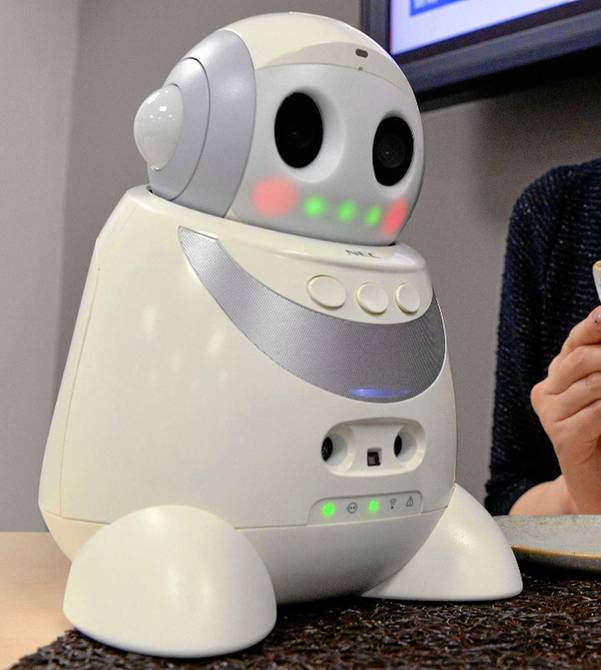
\includegraphics[width=0.235\linewidth,height=0.13\textheight,keepaspectratio]{images/intro/by_slide/s45_robots-de-compania_img07.png}%
    \hspace{0.008\linewidth}
    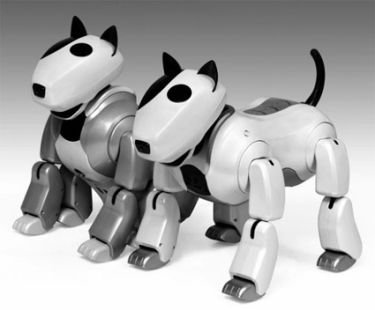
\includegraphics[width=0.235\linewidth,height=0.13\textheight,keepaspectratio]{images/intro/by_slide/s45_robots-de-compania_img08.jpeg}%
    \par\vspace{0.18em}

    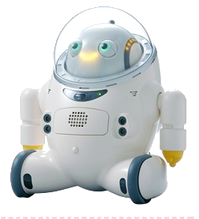
\includegraphics[width=0.19\linewidth,height=0.115\textheight,keepaspectratio]{images/intro/by_slide/s45_robots-de-compania_img09.jpeg}%
    \hspace{0.006\linewidth}
    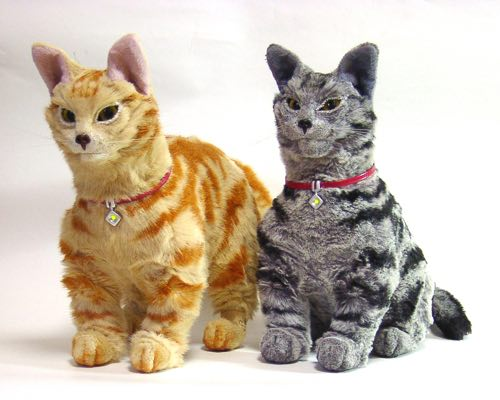
\includegraphics[width=0.19\linewidth,height=0.115\textheight,keepaspectratio]{images/intro/by_slide/s45_robots-de-compania_img10.jpeg}%
    \hspace{0.006\linewidth}
    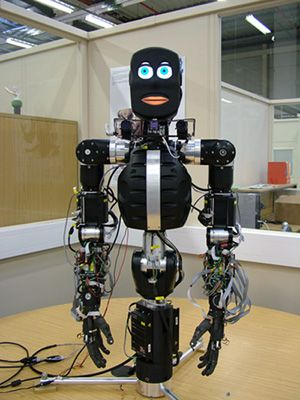
\includegraphics[width=0.19\linewidth,height=0.115\textheight,keepaspectratio]{images/intro/by_slide/s45_robots-de-compania_img11.jpeg}%
    \hspace{0.006\linewidth}
    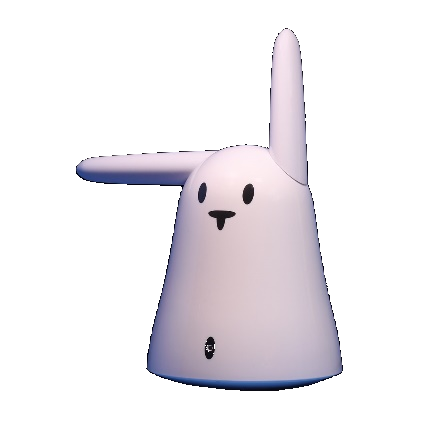
\includegraphics[width=0.19\linewidth,height=0.115\textheight,keepaspectratio]{images/intro/by_slide/s45_robots-de-compania_img12.png}%
    \hspace{0.006\linewidth}
    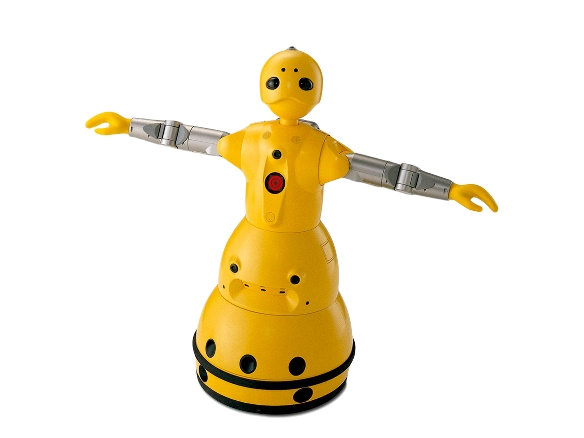
\includegraphics[width=0.19\linewidth,height=0.115\textheight,keepaspectratio]{images/intro/by_slide/s45_robots-de-compania_img13.png}%
    \par\vspace{0.2em}
  \end{center}
  \begin{itemize}
    \item Mejora del estado psicológico
    \item Fomento de la comunicación
  \end{itemize}
\end{frame}

% Página original 46
\begin{frame}{Robots de telepresencia}
  \small
  \begin{itemize}
    \item Conexión remota con otras personas $\rightarrow$ vídeo
    \item Algunos son móviles $\rightarrow$ guiado en el domicilio
    \item Sensación de conectividad con el exterior
  \end{itemize}
  \vspace{0.08em}
  \begin{center}
    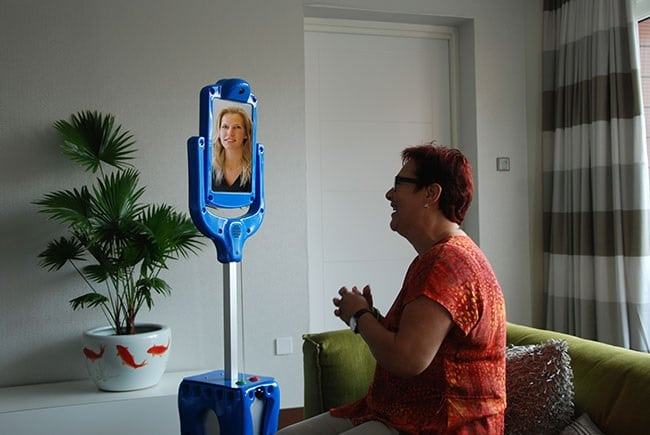
\includegraphics[width=0.6\linewidth,height=0.3\textheight,keepaspectratio]{images/intro/by_slide/s46_robots-de-telepresencia_img01.jpeg}%
    \hspace{0.01\linewidth}
    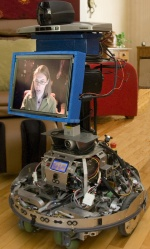
\includegraphics[width=0.6\linewidth,height=0.3\textheight,keepaspectratio]{images/intro/by_slide/s46_robots-de-telepresencia_img02.png}%
    \par\vspace{0.08em}
    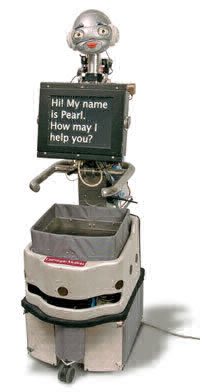
\includegraphics[width=0.6\linewidth,height=0.3\textheight,keepaspectratio]{images/intro/by_slide/s46_robots-de-telepresencia_img03.png}%
    \hspace{0.01\linewidth}
    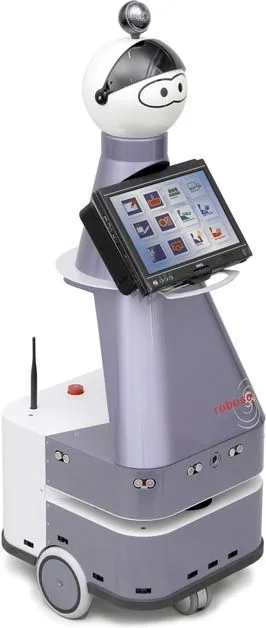
\includegraphics[width=0.6\linewidth,height=0.3\textheight,keepaspectratio]{images/intro/by_slide/s46_robots-de-telepresencia_img04.png}%
  \end{center}
\end{frame}

% Página original 47
\begin{frame}{Robots de servicio manipuladores}
  \small
  \begin{itemize}
    \item Con accesorios tipo brazo $\rightarrow$ manejo y transporte de objetos
    \item Soporte de actividades básicas de la vida diaria
  \end{itemize}
  \vspace{0.08em}
  \begin{center}
    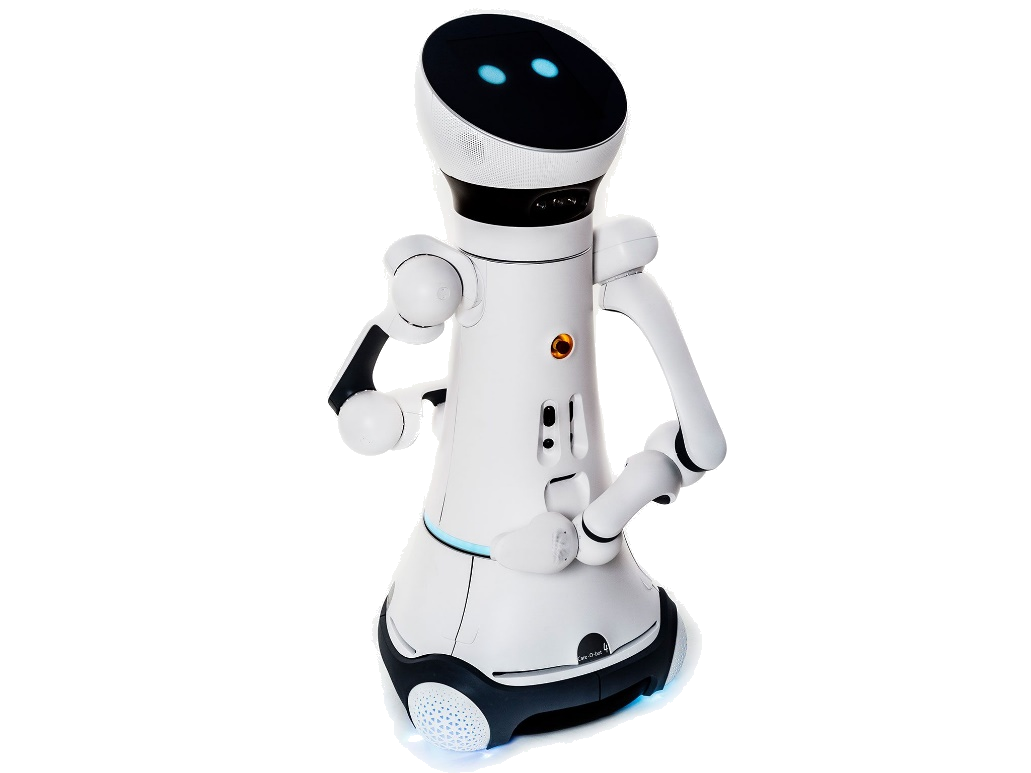
\includegraphics[width=0.6\linewidth,height=0.3\textheight,keepaspectratio]{images/intro/by_slide/s47_robots-de-servicio-manipuladores_img01.png}%
    \hspace{0.01\linewidth}
    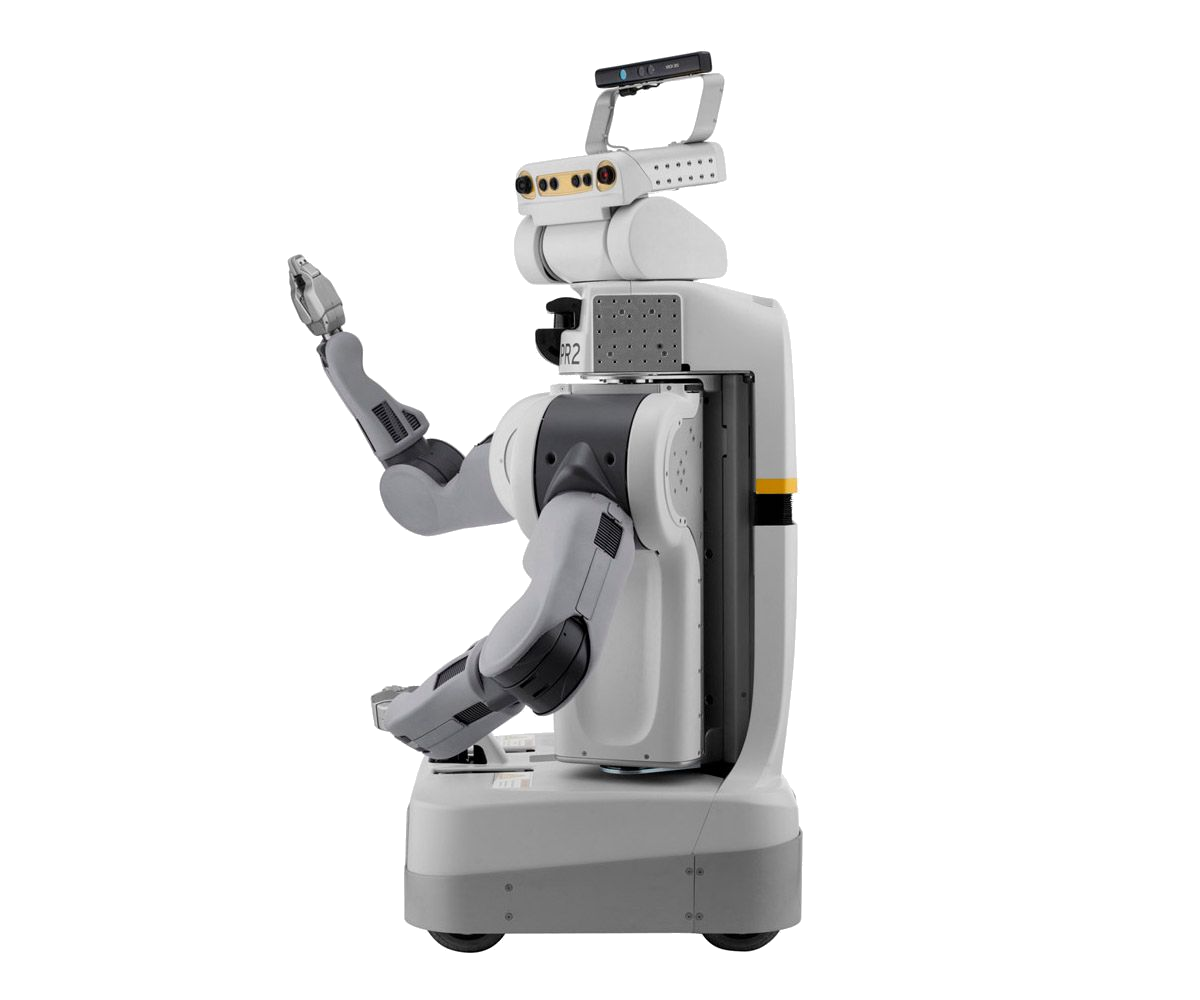
\includegraphics[width=0.6\linewidth,height=0.3\textheight,keepaspectratio]{images/intro/by_slide/s47_robots-de-servicio-manipuladores_img02.jpeg}%
    \par\vspace{0.08em}
    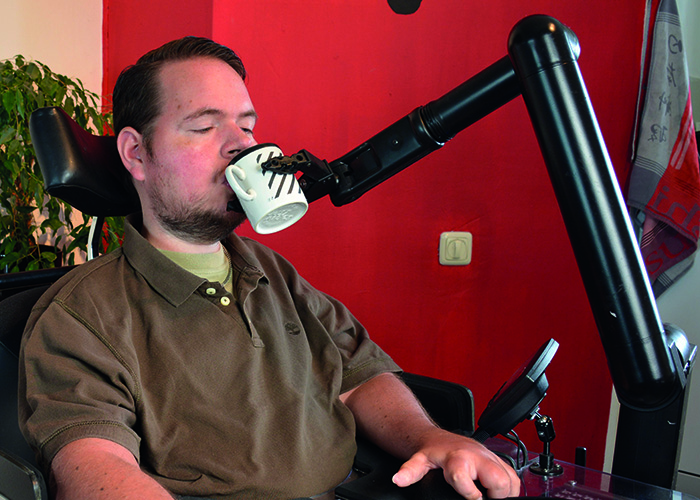
\includegraphics[width=0.6\linewidth,height=0.3\textheight,keepaspectratio]{images/intro/by_slide/s47_robots-de-servicio-manipuladores_img03.jpeg}%
    \hspace{0.01\linewidth}
    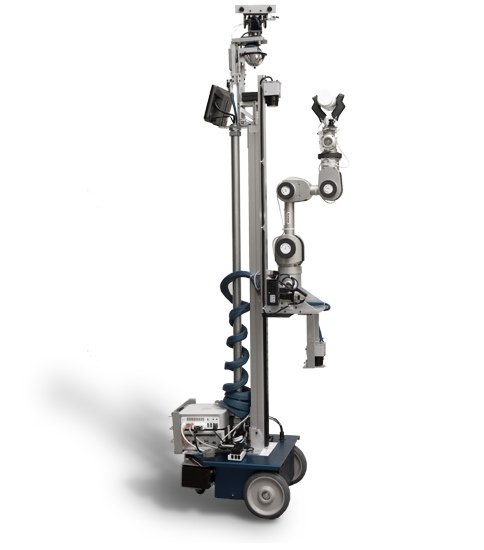
\includegraphics[width=0.6\linewidth,height=0.3\textheight,keepaspectratio]{images/intro/by_slide/s47_robots-de-servicio-manipuladores_img04.png}%
  \end{center}
\end{frame}

% Página original 48
\begin{frame}{Robots de asistencia a la movilidad}
  \small
  \begin{itemize}
    \item Asistencia a la movilidad
    \item Sin capacidades sociales
  \end{itemize}
  \vspace{0.08em}
  \begin{center}
    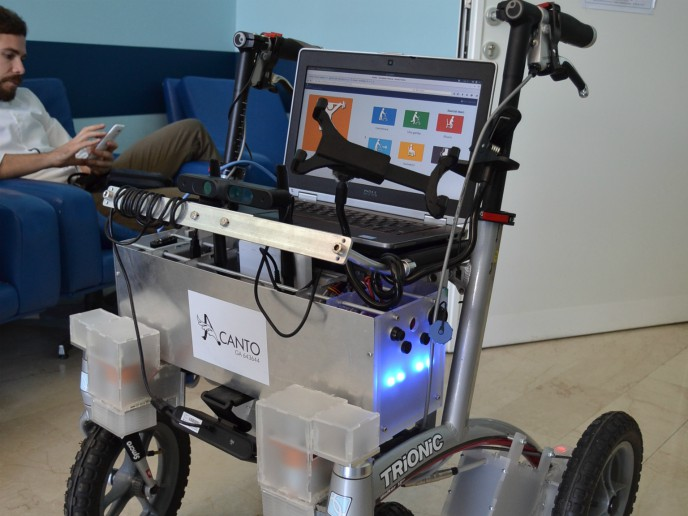
\includegraphics[width=0.48\linewidth,height=0.3\textheight,keepaspectratio]{images/intro/by_slide/s48_robots-de-asistencia-a-la-movilidad_img01.jpeg}%
    \hspace{0.01\linewidth}
    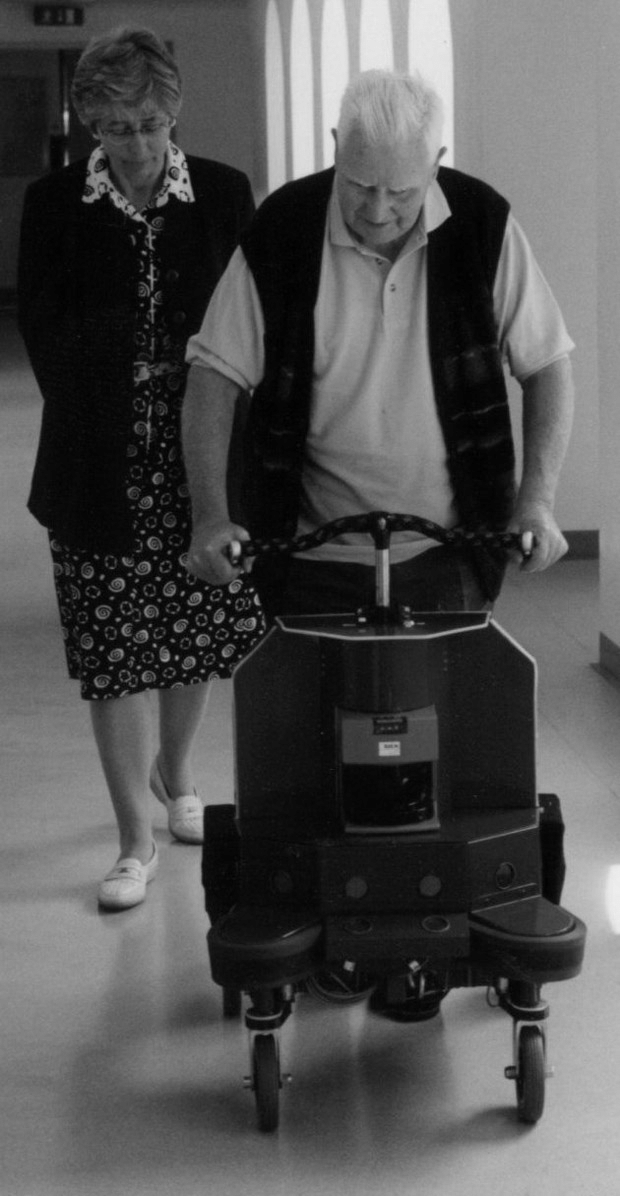
\includegraphics[width=0.48\linewidth,height=0.39\textheight,keepaspectratio]{images/intro/by_slide/s48_robots-de-asistencia-a-la-movilidad_img02.png}%
    \par\vspace{0.08em}
    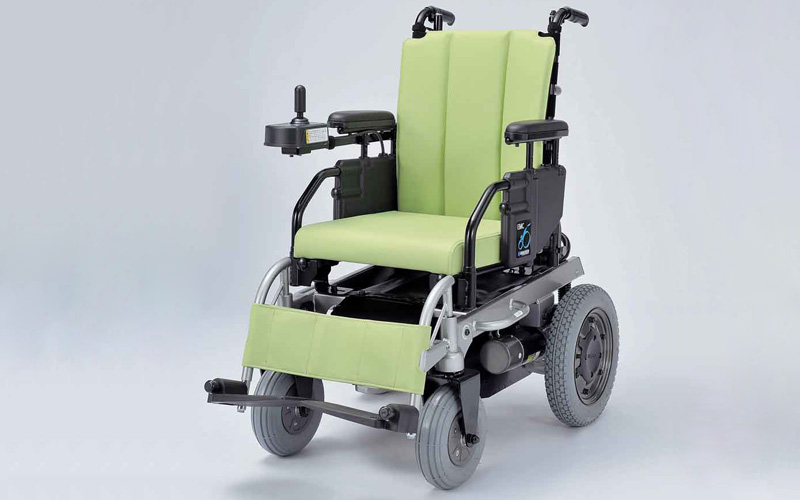
\includegraphics[width=0.48\linewidth,height=0.3\textheight,keepaspectratio]{images/intro/by_slide/s48_robots-de-asistencia-a-la-movilidad_img03.jpeg}%
    \hspace{0.01\linewidth}
    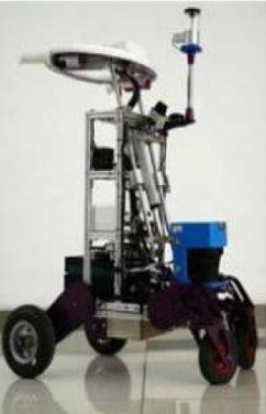
\includegraphics[width=0.48\linewidth,height=0.3\textheight,keepaspectratio]{images/intro/by_slide/s48_robots-de-asistencia-a-la-movilidad_img04.png}%
  \end{center}
\end{frame}

\begin{frame}{Robots de asistencia a la movilidad}

  \begin{center}
    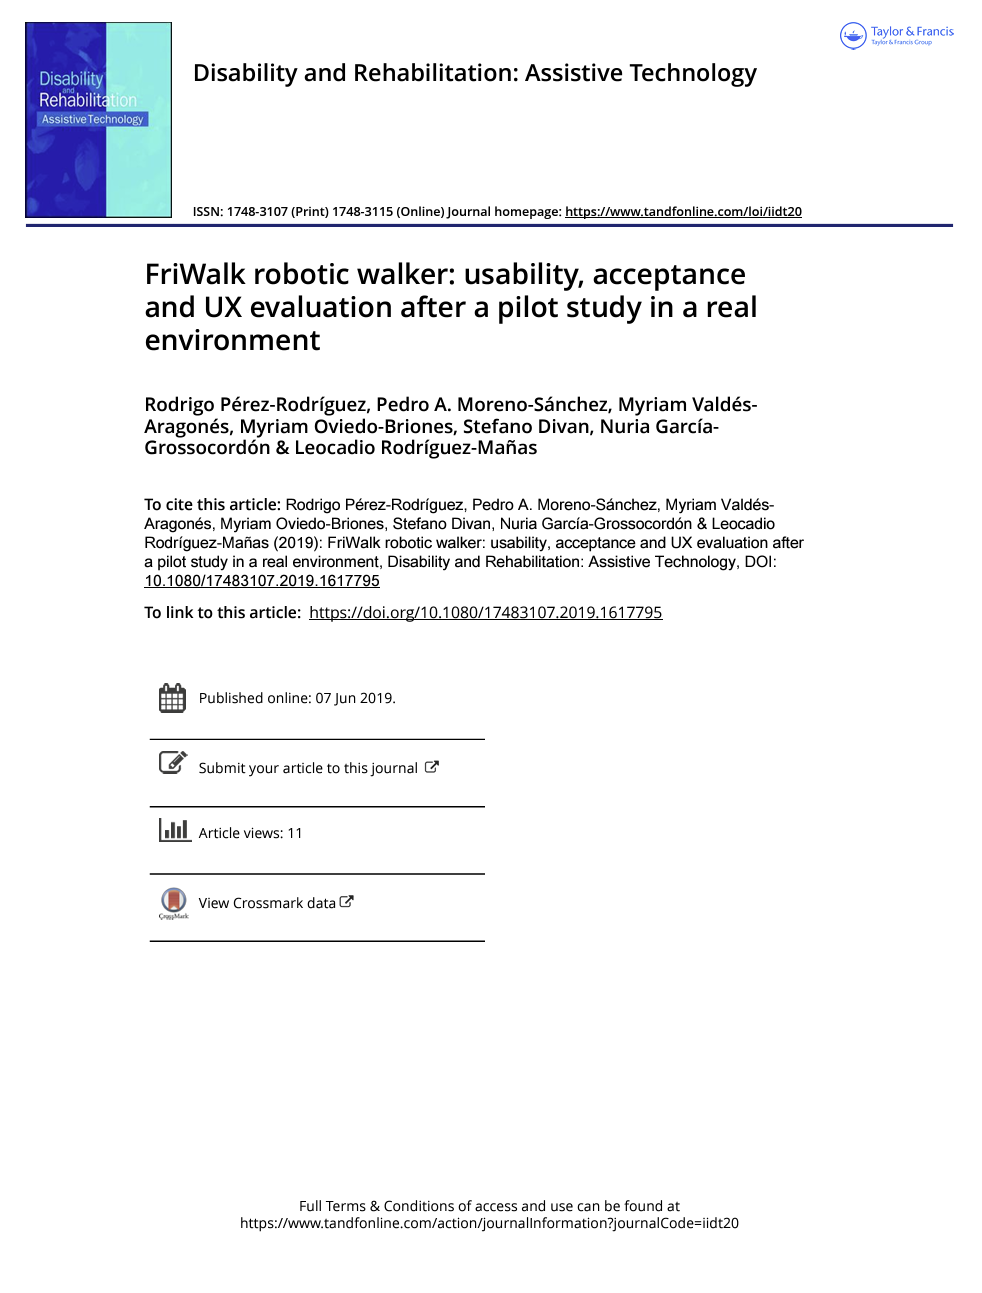
\includegraphics[width=1\linewidth,height=1\textheight,keepaspectratio]{images/intro/by_slide/s49_robots-de-asistencia-a-la-movilidad_img01.png}
  \end{center}
\end{frame}


% Página original 51
\begin{frame}{Robots domésticos}
  \small
  \begin{itemize}
    \item Apoyo en la realización de tareas domésticas $\rightarrow$ limpieza, cocina, higiene, etc.
  \end{itemize}
  \begin{center}
    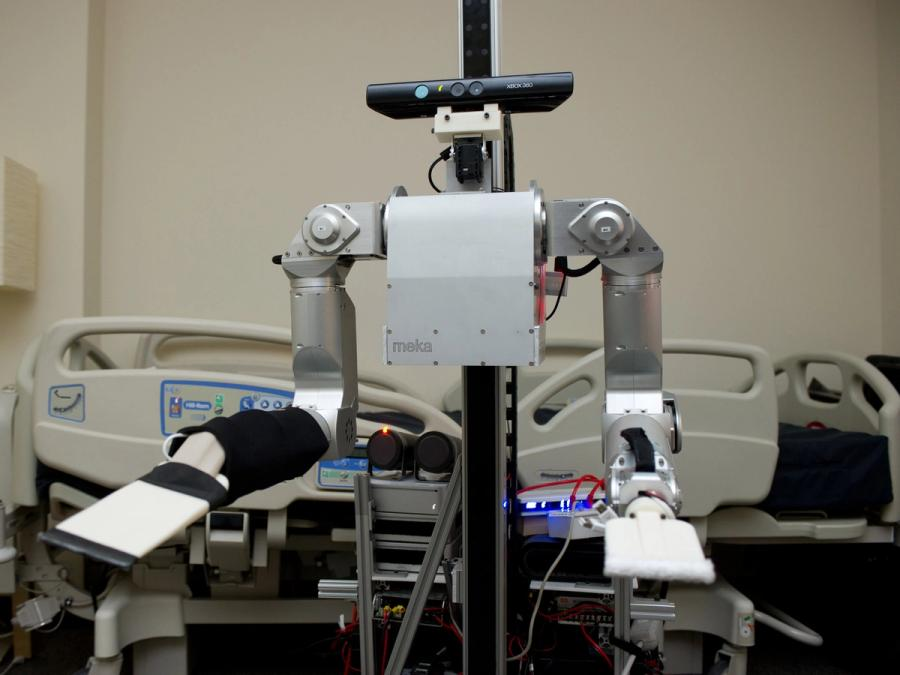
\includegraphics[width=0.6\linewidth,height=0.3\textheight,keepaspectratio]{images/intro/by_slide/s51_robots-domesticos_img01.jpeg}%
    \hspace{0.01\linewidth}
    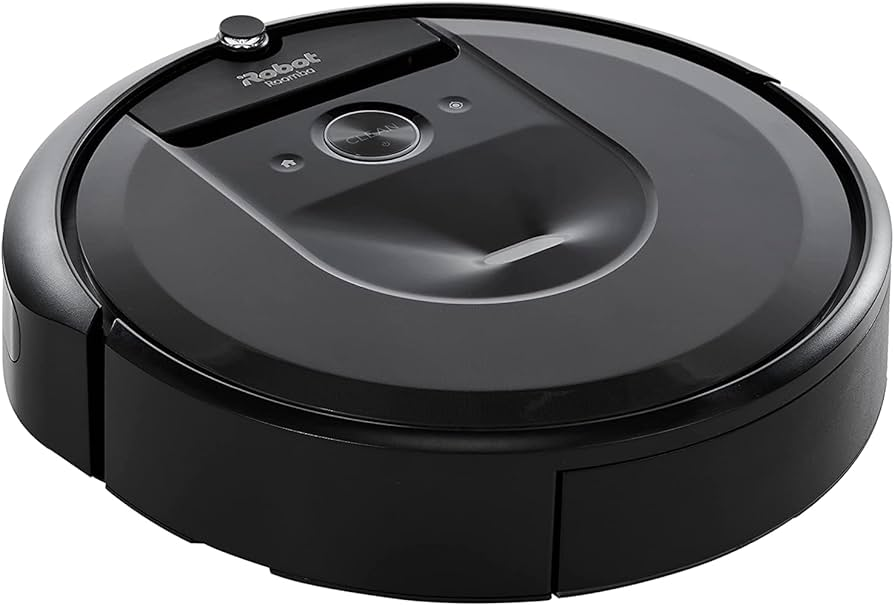
\includegraphics[width=0.6\linewidth,height=0.3\textheight,keepaspectratio]{images/intro/by_slide/s51_robots-domesticos_img02.jpeg}%
    \par\vspace{0.25em}
  \end{center}
\end{frame}

% Página original 52
\begin{frame}{Robots de monitorización}
  \small
  \begin{center}
    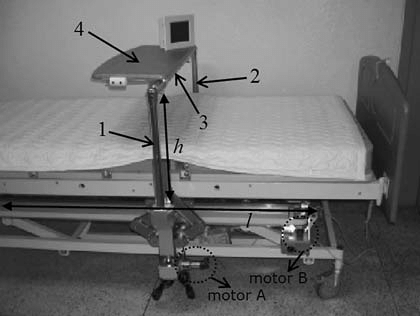
\includegraphics[width=1\linewidth,height=0.8\textheight,keepaspectratio]{images/intro/by_slide/s52_robots-de-monitorizacion_img01.png}%
    \par\vspace{0.25em}
  \end{center}

\end{frame}

% Página original 53
\begin{frame}{Robots recreacionales}
  \small
  \begin{center}
    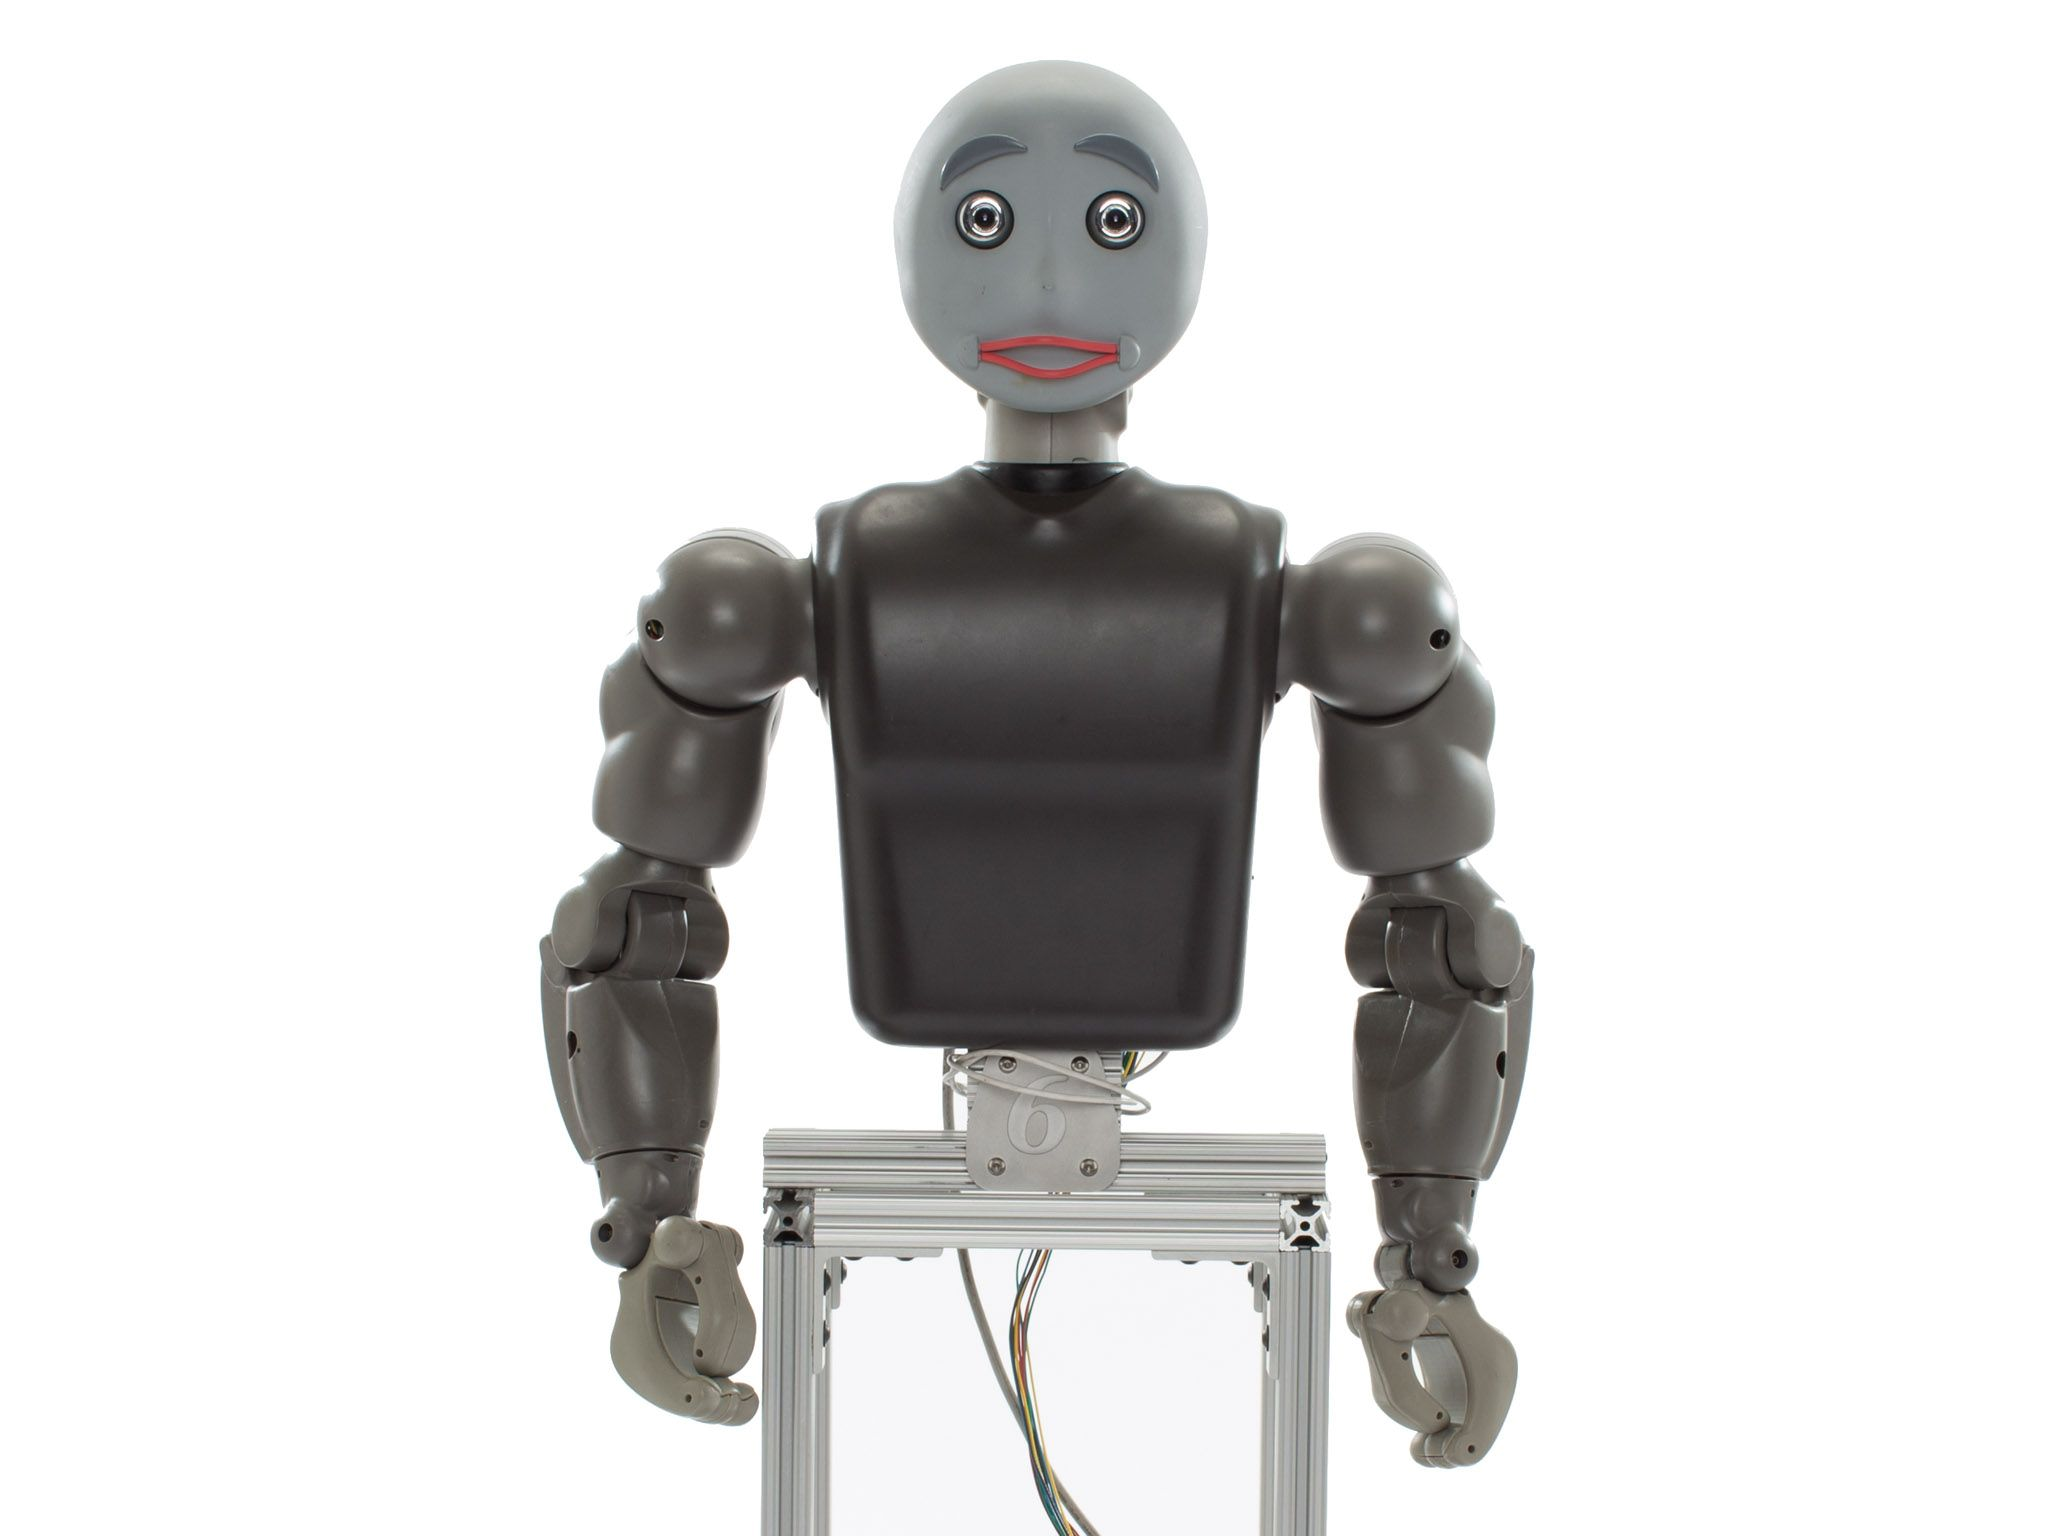
\includegraphics[width=0.8\linewidth,height=0.4\textheight,keepaspectratio]{images/intro/by_slide/s53_robots-recreacionales_img01.png}%
    \hspace{0.01\linewidth}
    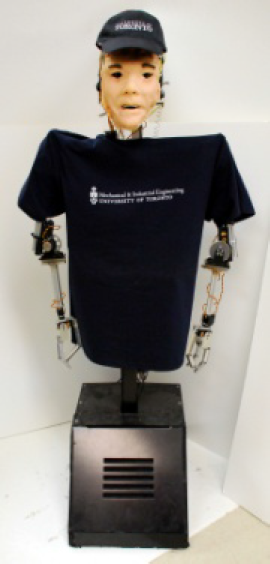
\includegraphics[width=0.8\linewidth,height=0.4\textheight,keepaspectratio]{images/intro/by_slide/s53_robots-recreacionales_img02.png}%
    \par\vspace{0.25em}
  \end{center}
\end{frame}

% Página original 54
\begin{frame}{Otros: ADELA}
  \small
  \vspace{0.25em}
  \begin{center}
    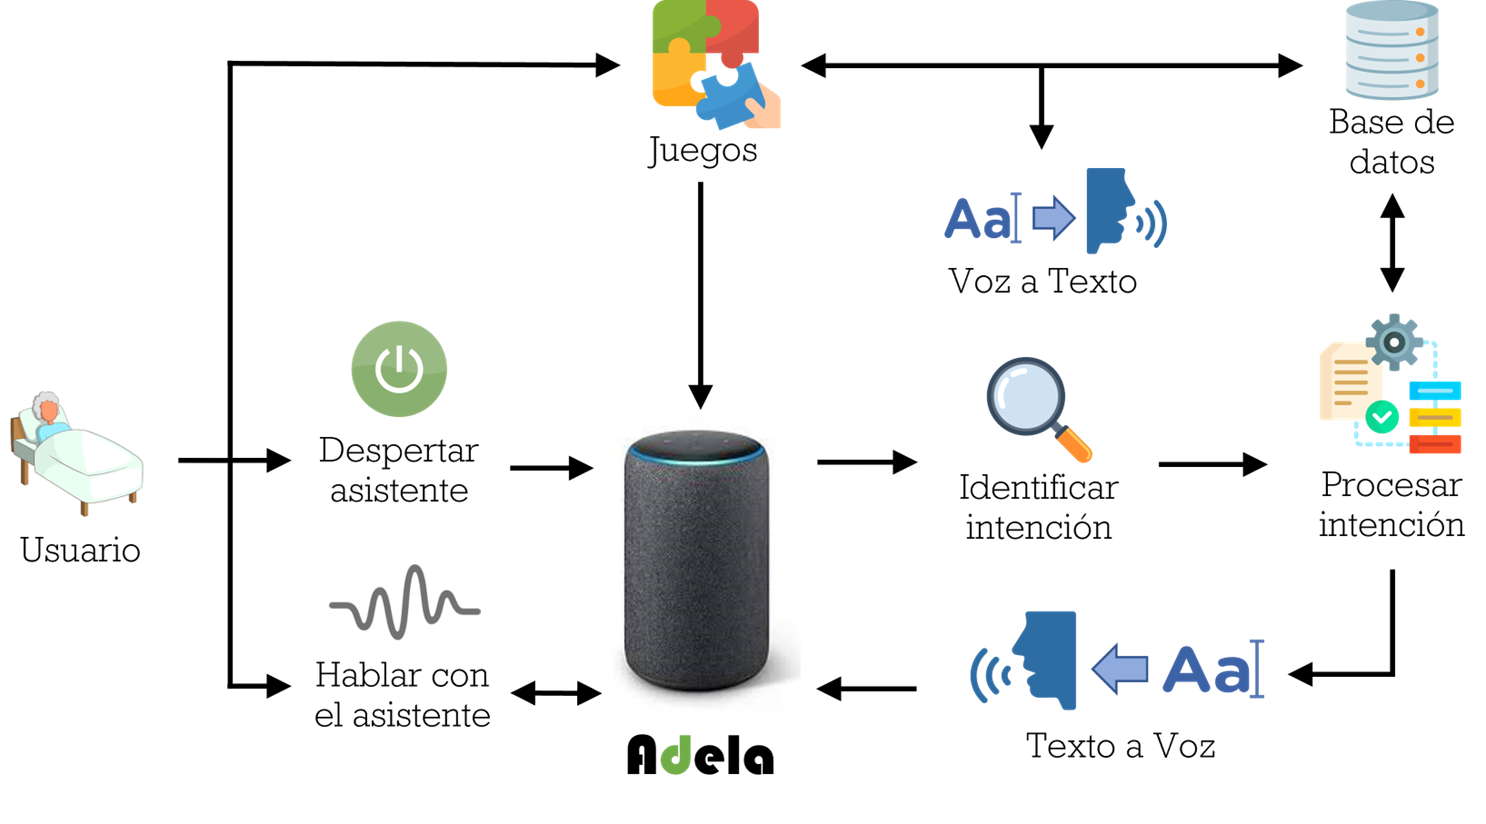
\includegraphics[width=0.7\linewidth,height=1\textheight,keepaspectratio]{images/intro/by_slide/s54_otros-adela_img01.png}%
    \hspace{0.01\linewidth}
    
\includegraphics[width=0.7\linewidth,height=0.4\textheight,keepaspectratio]{images/intro/by_slide/s54_otros-adela_img02.png}%
    \par\vspace{0.25em}
  \end{center}
  \vfill
\end{frame}

% Página original 55
\begin{frame}{Otros: ADELA}
  \small
  \vspace{0.25em}
  \begin{center}
    % \par\vspace{0.25em}
    
\includegraphics[width=0.32\linewidth,height=0.15\textheight,keepaspectratio]{images/intro/by_slide/s55_otros-adela_img05.png}%
    \par\vspace{0.25em}
    
\includegraphics[width=1\linewidth,height=0.5\textheight,keepaspectratio]{images/intro/by_slide/s55_otros-adela_img02.png}%
    \hspace{0.01\linewidth}
    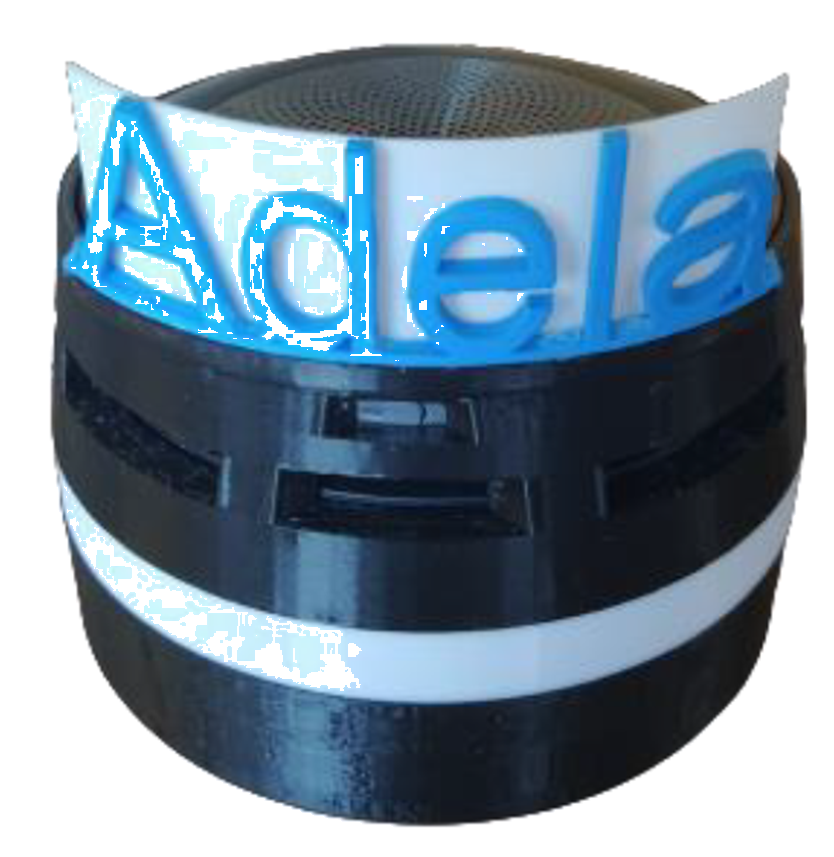
\includegraphics[width=1\linewidth,height=0.5\textheight,keepaspectratio]{images/intro/by_slide/s55_otros-adela_img03.png}%
    
  \end{center}
  \begin{itemize}
    \item SUS $\rightarrow$ 75/10
    \item CUQ $\rightarrow$ 85/10
  \end{itemize}
\end{frame}


% Página original 57
\begin{frame}{Otros: Adela}
  \small

  \begin{itemize}
    \item Estudio preliminar (40 personas mayores hospitalizadas):
    \begin{itemize}
      \item Ningún paciente del GI desarrolló delirium ni ninguna de las complicaciones asociadas a él
      \item Barthel al alta $\rightarrow$ 71 en GI vs. 46.8 en GC
      \item Duración de la estancia $\rightarrow$ 4.71 días en GI vs. 6.68 en GC
    \end{itemize}
  \end{itemize}
  \begin{center}
    
\includegraphics[width=0.48\linewidth,height=0.5\textheight,keepaspectratio]{images/intro/by_slide/s57_estudio-preliminar-40-personas-mayores-hospitalizadas-ningun_img03.png}%
    \hspace{0.01\linewidth}
    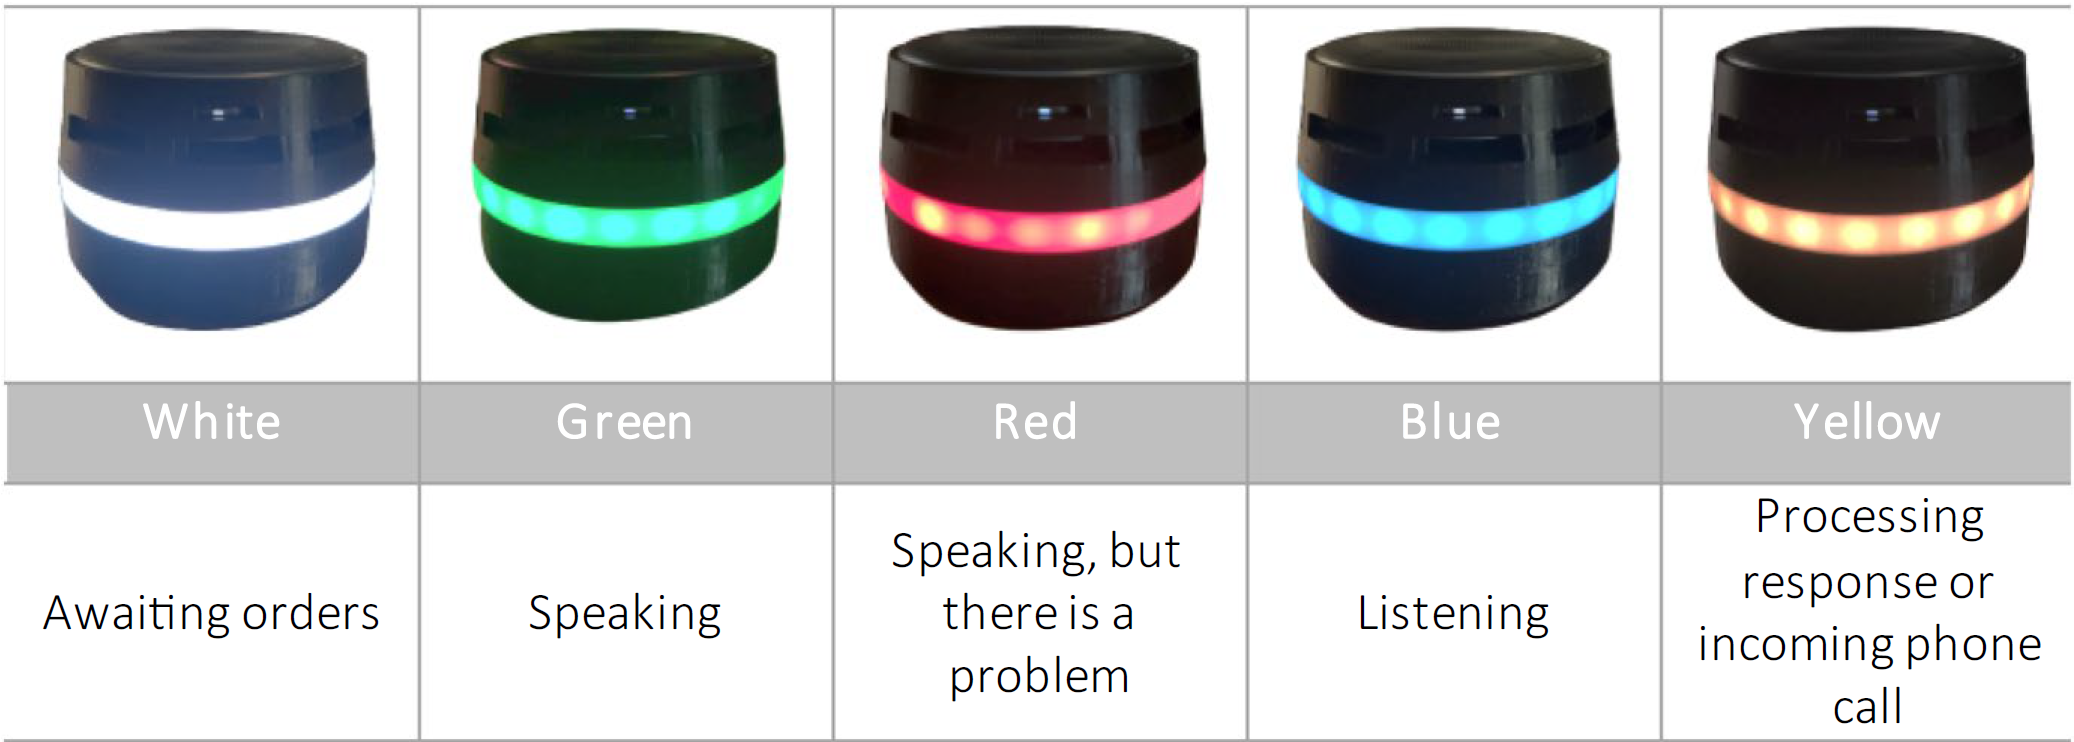
\includegraphics[width=0.48\linewidth,height=1\textheight,keepaspectratio]{images/intro/by_slide/s57_estudio-preliminar-40-personas-mayores-hospitalizadas-ningun_img04.png}%
    \par\vspace{0.25em}
  \end{center}
\end{frame}


\begin{frame}{Otros: Adela}

  \begin{center}
    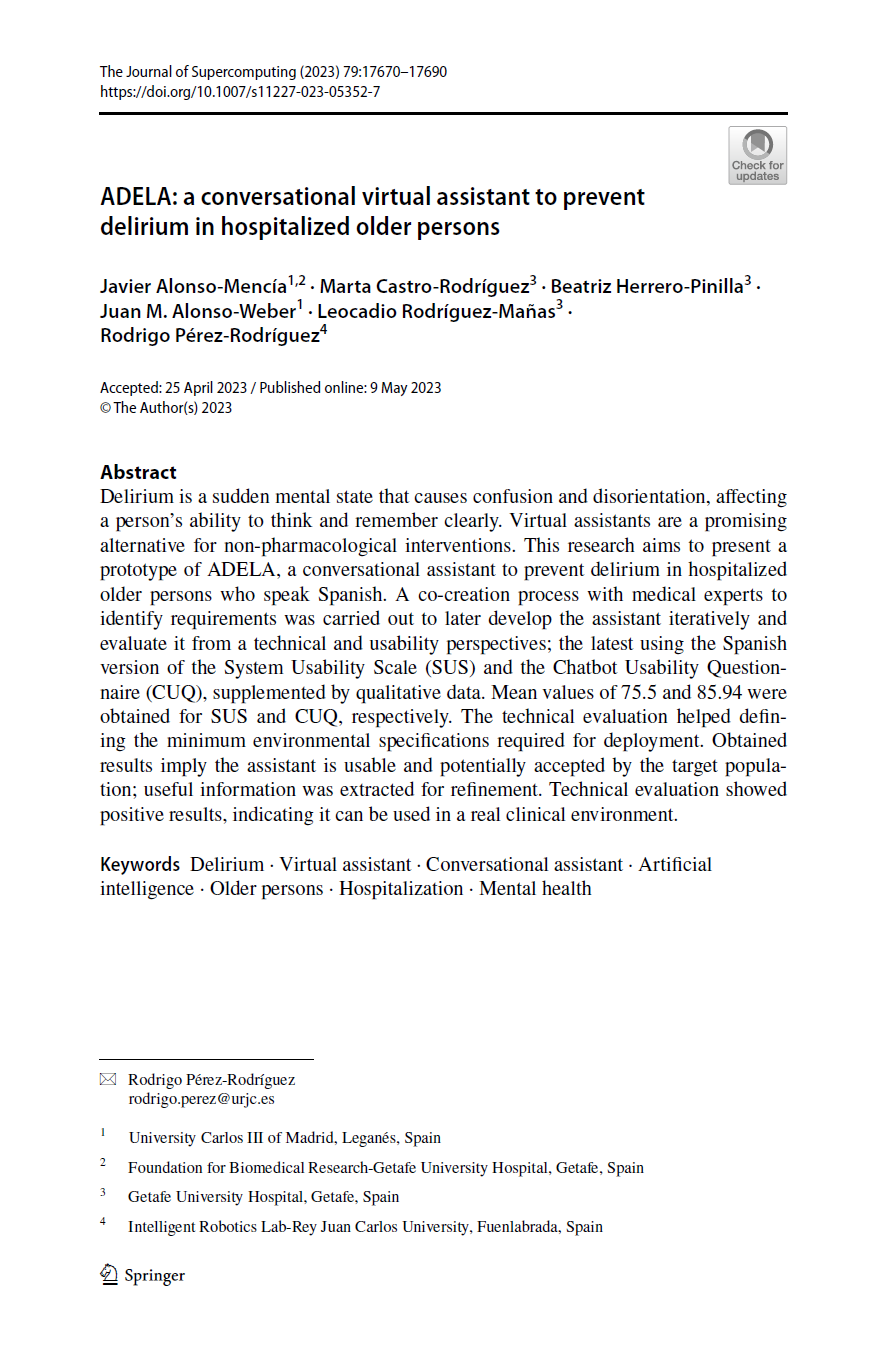
\includegraphics[width=1\linewidth,height=0.9\textheight,keepaspectratio]{images/intro/by_slide/s56_otros-adela_img06.png}%

  \end{center}
\end{frame}


% Página original 58
\section{Conclusiones}


% Página original 59
\begin{frame}{Qué puede aportar la robótica}
  \small
  \begin{itemize}
    \item Asistencia física y emocional
    \item Compañía (evitar la sensación de soledad)
    \item Estimulación física y cognitiva
    \item Reducción de la carga de trabajo a cuidadores
    \item Disminución de costes de atención
    \item ...
  \end{itemize}
  \begin{center}
    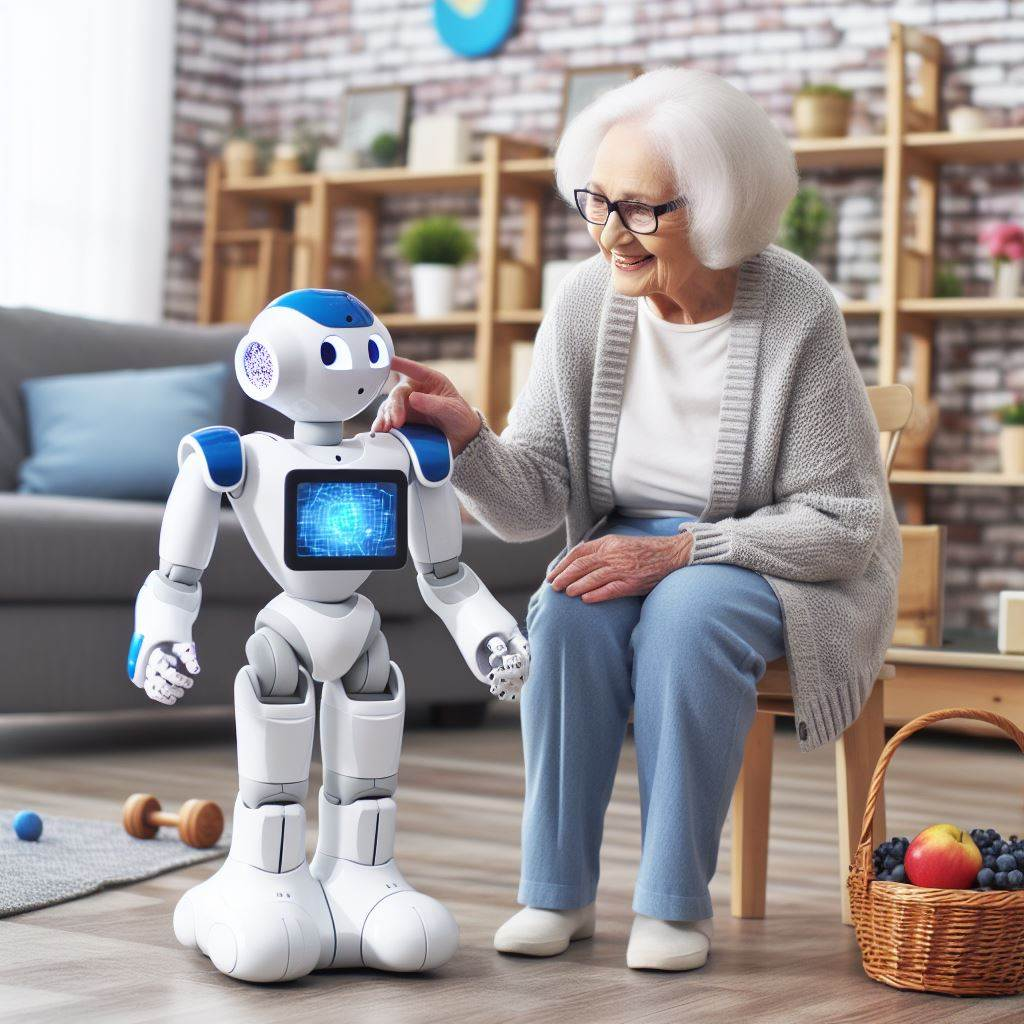
\includegraphics[width=0.6\linewidth,height=0.3\textheight,keepaspectratio]{images/intro/by_slide/s59_que-puede-aportar-la-robotica_img01.png}%
    \hspace{0.01\linewidth}
    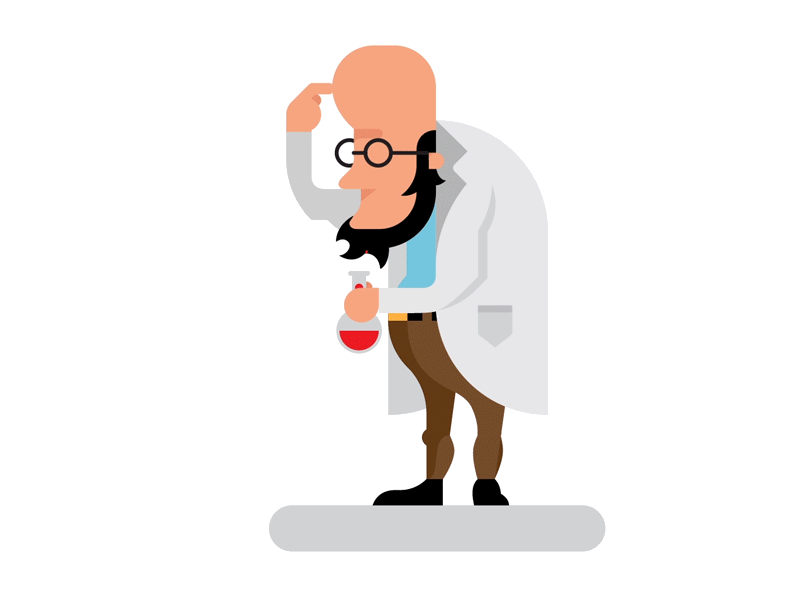
\includegraphics[width=0.6\linewidth,height=0.3\textheight,keepaspectratio]{images/intro/by_slide/s59_que-puede-aportar-la-robotica_img02.png}%
    \par\vspace{0.25em}
  \end{center}
\end{frame}

% Página original 60
\begin{frame}{Retos}
  \small
  \begin{itemize}
    \item Coste de los robots
    \item Aceptación, tanto por parte de personas mayores como de profesionales y cuidadores
    \item Necesidades de formación
    \item ...
  \end{itemize}
  \begin{center}
    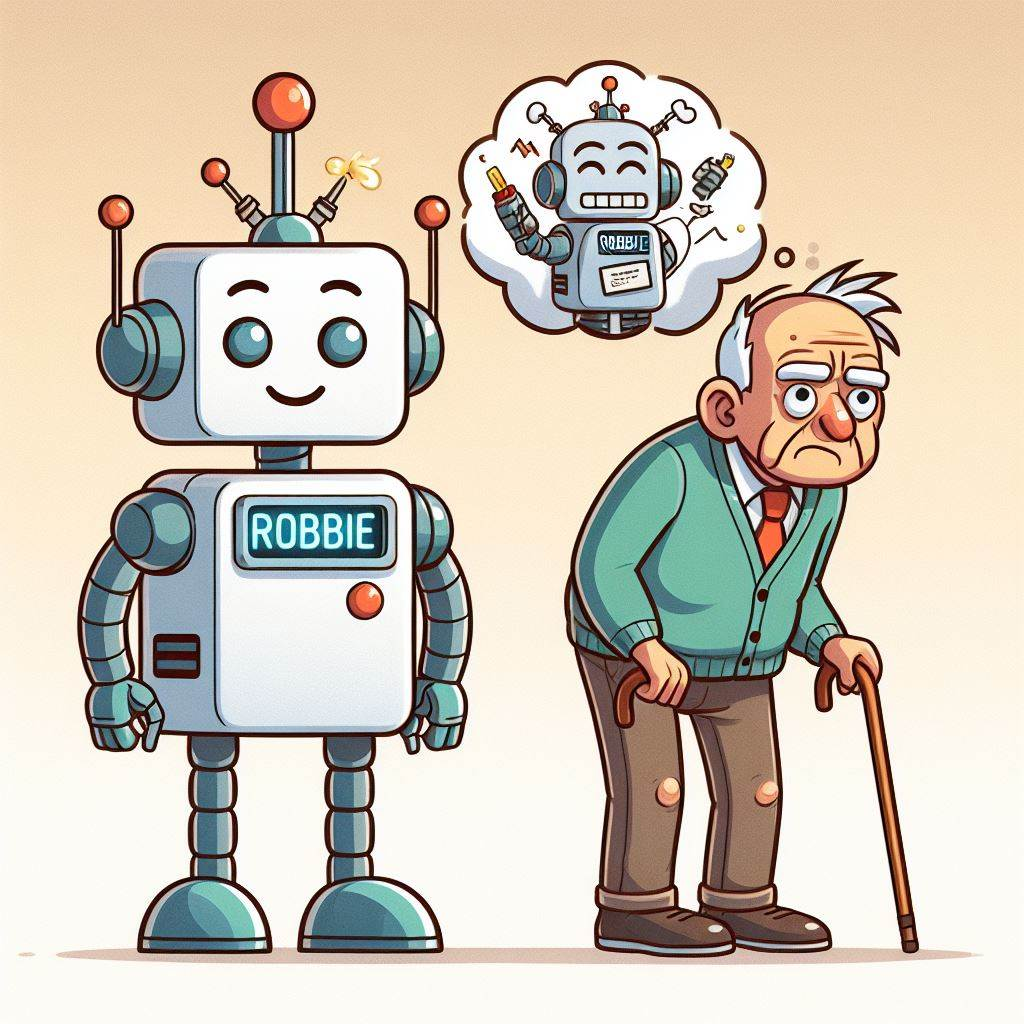
\includegraphics[width=0.6\linewidth,height=0.3\textheight,keepaspectratio]{images/intro/by_slide/s60_retos_img01.png}%
    \hspace{0.01\linewidth}
    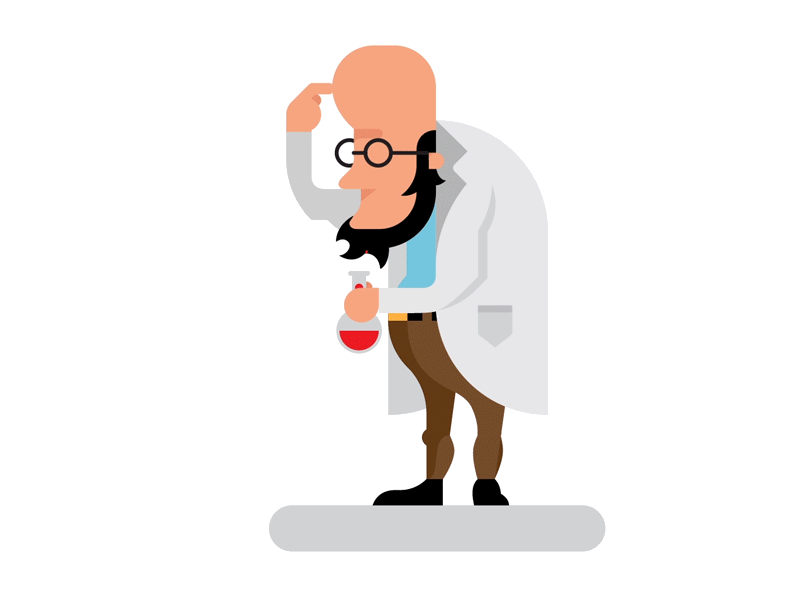
\includegraphics[width=0.6\linewidth,height=0.3\textheight,keepaspectratio]{images/intro/by_slide/s60_retos_img02.png}%
  \end{center}
\end{frame}

% Página original 61
\begin{frame}{Uncanny valley}
  \small
  \vspace{0.25em}
  \begin{center}
    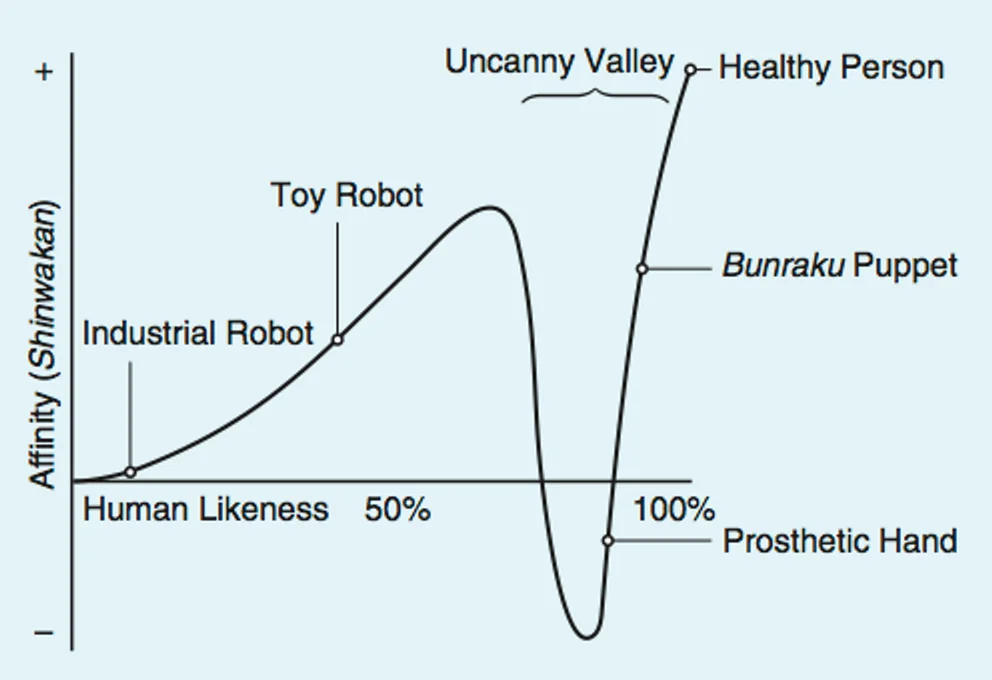
\includegraphics[width=0.78\linewidth,height=0.36\textheight,keepaspectratio]{images/intro/by_slide/s61_uncanny-valley_img01.png}%
    \par\vspace{0.25em}
  \end{center}
  \begin{itemize}
    \item Mashahiro Mori → 1970
    \item A medida que un robot se parece más a un humano, genera más empatía… hasta que se vuelve demasiado parecido, pero no del todo humano, y entonces provoca rechazo o incomodidad
  \end{itemize}
\end{frame}

% Página original 62
\begin{frame}{Uncanny valley}
  \small
  \vspace{0.25em}
  \begin{center}
    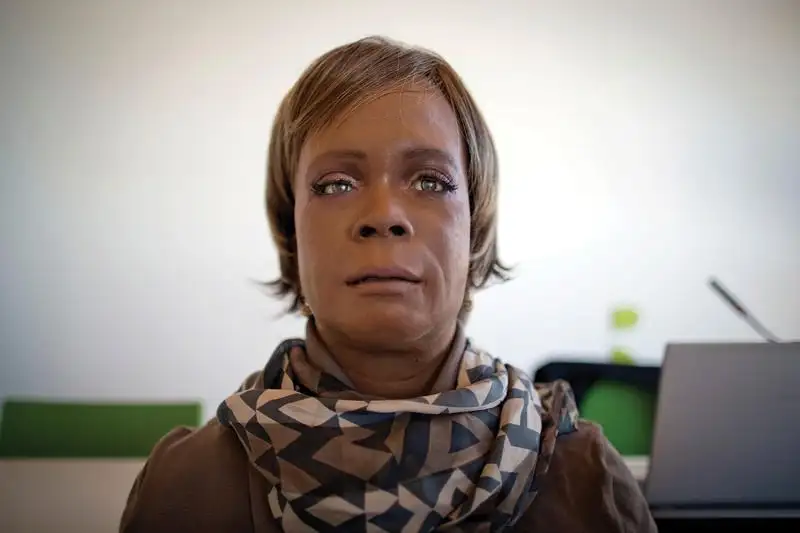
\includegraphics[width=0.78\linewidth,height=0.36\textheight,keepaspectratio]{images/intro/by_slide/s62_uncanny-valley_img01.png}%
    \par\vspace{0.25em}
  \end{center}
  \begin{itemize}
    \item ¿Por qué se produce?
    \begin{itemize}
      \item Posibles incongruencias en el movimiento de la cara (movimientos percibidos como antinaturales)
      \item Sensación de que el robot es una persona extraña, enferma, o incluso muerta
      \item Disonancia cognitiva por la dicotomía vivo-artificial
    \end{itemize}
  \end{itemize}
\end{frame}

% Página original 63
\begin{frame}{Uncanny valley}
  \small
  \begin{itemize}
    \item Importante evitar este efecto en el ámbito de la robótica asistencial
    \item Uso de diseños no realistas que no crucen el valle
    \item Geminoid HI-2 vs. TiaGo:
  \begin{center}
  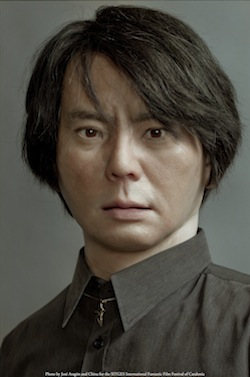
\includegraphics[width=1\linewidth,height=0.6\textheight,keepaspectratio]{images/intro/by_slide/s63_uncanny-valley_img01.png}%
  \hspace{0.01\linewidth}
  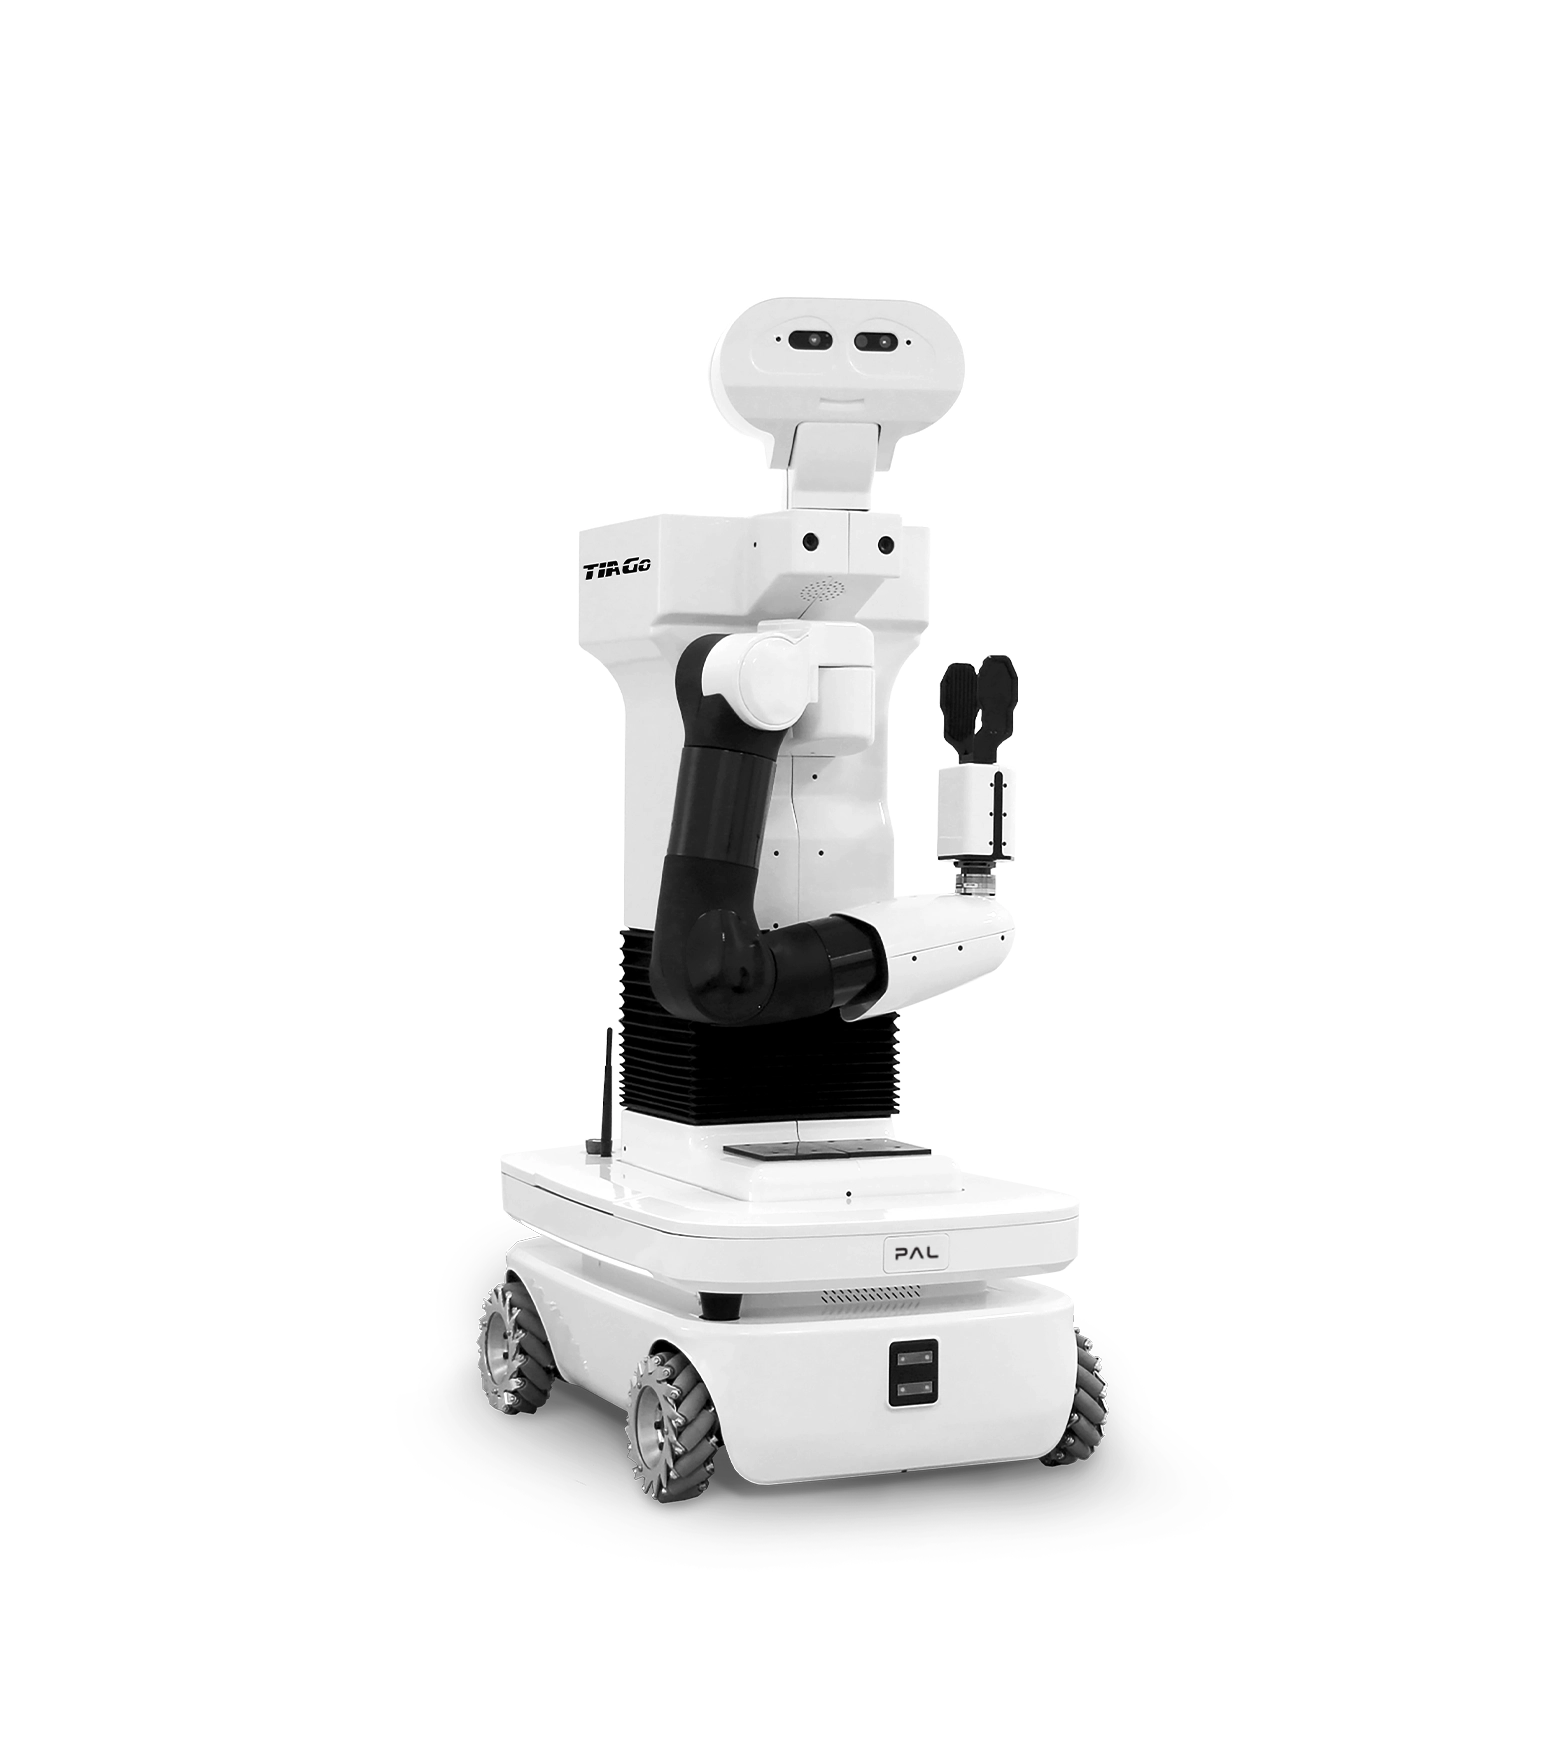
\includegraphics[width=1\linewidth,height=0.7\textheight,keepaspectratio]{images/intro/by_slide/s63_uncanny-valley_img02.png}%
  \par\vspace{0.25em}
  \end{center}
  \end{itemize}
\end{frame}

% Página original 64
% \section{La llegada de los LLMs}
% \begin{frame}{La llegada de la IA generativa}
%   \small
%   \vspace{0.25em}
%   \begin{center}
%     \includegraphics[width=0.32\linewidth,height=0.15\textheight,keepaspectratio]{images/intro/by_slide/s64_la-llegada-de-los-llms_img01.png}%
%     \hfill
%     \includegraphics[width=0.32\linewidth,height=0.15\textheight,keepaspectratio]{images/intro/by_slide/s64_la-llegada-de-los-llms_img02.png}%
%     \hfill
%     \includegraphics[width=0.32\linewidth,height=0.15\textheight,keepaspectratio]{images/intro/by_slide/s64_la-llegada-de-los-llms_img03.png}%
%     \par\vspace{0.25em}
%     \includegraphics[width=0.32\linewidth,height=0.15\textheight,keepaspectratio]{images/intro/by_slide/s64_la-llegada-de-los-llms_img04.png}%
%     \hfill
%     \includegraphics[width=0.32\linewidth,height=0.15\textheight,keepaspectratio]{images/intro/by_slide/s64_la-llegada-de-los-llms_img05.jpeg}%
%     \hfill
%     \par\vspace{0.25em}
%   \end{center}
%   \vfill
% \end{frame}

% Página original 65
\begin{frame}{La llegada de la IA generativa}
  \small
  \begin{columns}[c,onlytextwidth]
    \begin{column}{0.52\textwidth}
      \begin{itemize}
        \item Planificación
        \item Interacción natural humano-robot
        \item Apoyo cognitivo
        \item Personalización del cuidado:
        \item Análisis de rutinas
        \item Identificación de necesidades en tiempo real
        \item Aprendizaje continuo
        \item ...
      \end{itemize}
    \end{column}
    \begin{column}{0.48\textwidth}
      \centering
      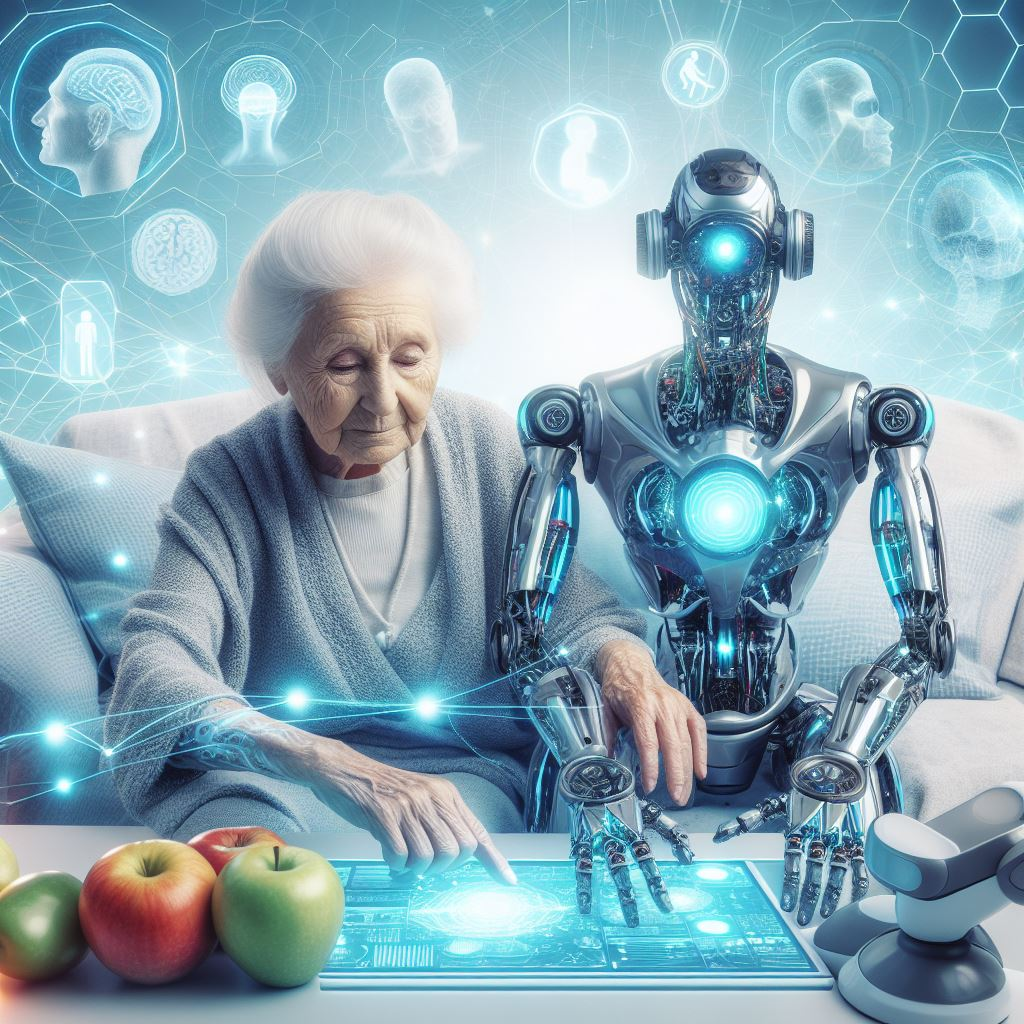
\includegraphics[width=0.98\linewidth,height=0.7\textheight,keepaspectratio]{images/intro/by_slide/s65_la-llegada-de-los-llms_img01.jpeg}
    \end{column}
  \end{columns}
\end{frame}



\end{document}
